\chapter{ピクセル解析ツールと読み出し試験のデモンストレーション}
品質試験項目の1つである読み出し試験のデモンストレーションを学内実験室にて行った。
デモンストレーションの内容としては、4章で述べた2月にCERNで行ったチュートリアルとほぼ同じ内容である。
この章の前半では開発したツールと試験で使用するソフトウェア、ハードウェアについて説明し、後にデモンストレーションの内容、各ソフトウェアの機能確認について述べる。

\section{ピクセル解析ツールの開発}
品質試験における読み出し試験では、3章で述べたようにモジュールの性能確認のためにピクセル解析を行う。
これを円滑に行うために、ピクセル解析ツールを開発した。また開発した解析ツールをローカルデータベースシステムに組み込んだ。
このツールについての詳細を以下に示す。

\subsection{概要}
YARRで読み出し試験を行った場合、結果ファイル及びディレクトリは各試験項目ごとにわかれて生成される。
また各結果ファイルにはモジュール上の全ピクセル結果がJSONの形で保存されている。

一方、ピクセル解析において、いくつかの試験結果を統一的に扱い、各ピクセルごとに解析を行う必要がある。
そこで、開発した解析ツールでは複数の結果ファイルを1つに統合し、ピクセルごとの解析処理を単純化する役割を担っている。
開発にはPythonとC++を用いた。またCERNが提供している解析フレームワークであるROOT\cite{5-5}を使用し、いくつかの試験データの統一ファイルとして、ROOT内部機能であるTreeを使用した。
このファイル統合処理のイメージを図\ref{analysis_tool_motivation}に示す。

\begin{figure}[bpt]\centering
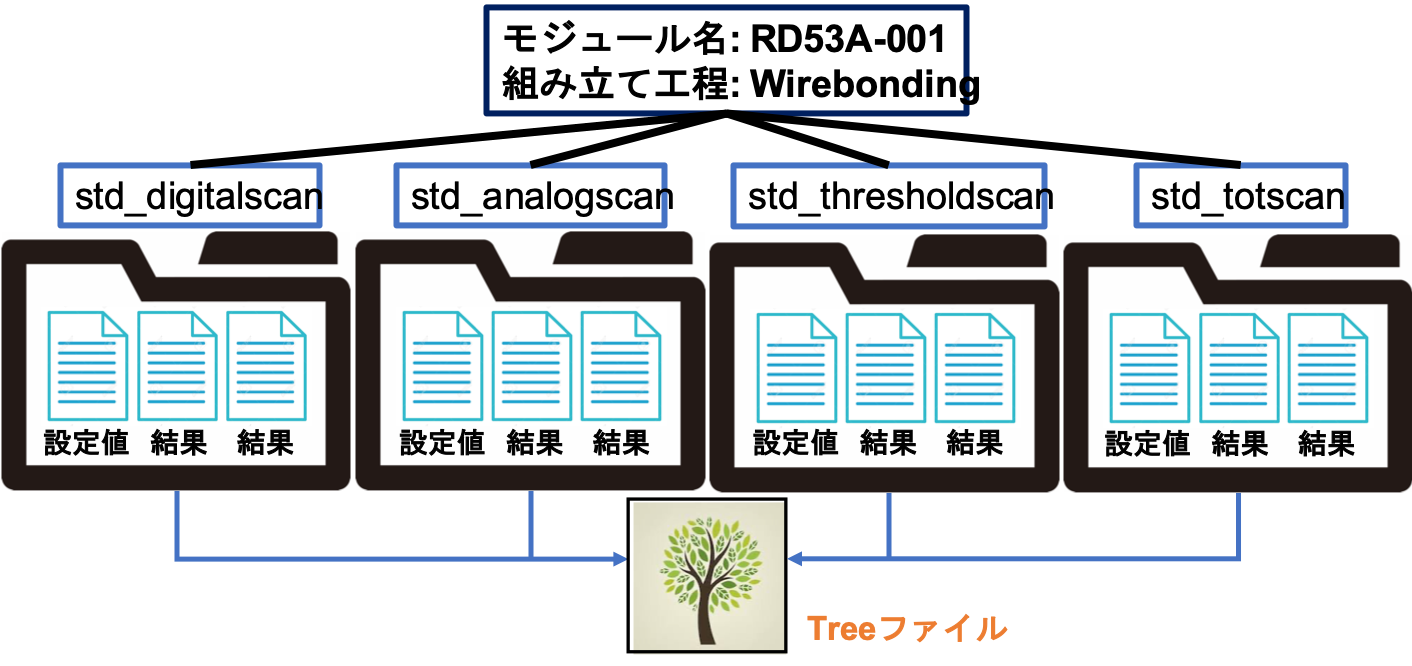
\includegraphics[width=12cm]{analysis_tool_motivation}
\caption[ピクセル解析ツール開発の動機]{ピクセル解析ツール開発の動機}
\label{analysis_tool_motivation}
\end{figure}

実際に作ったTreeファイルと、データ構造のイメージを図\ref{analysis_tool_tree}に示す。

\begin{figure}[bpt]
  \begin{center}
  \begin{minipage}{0.4\hsize}
    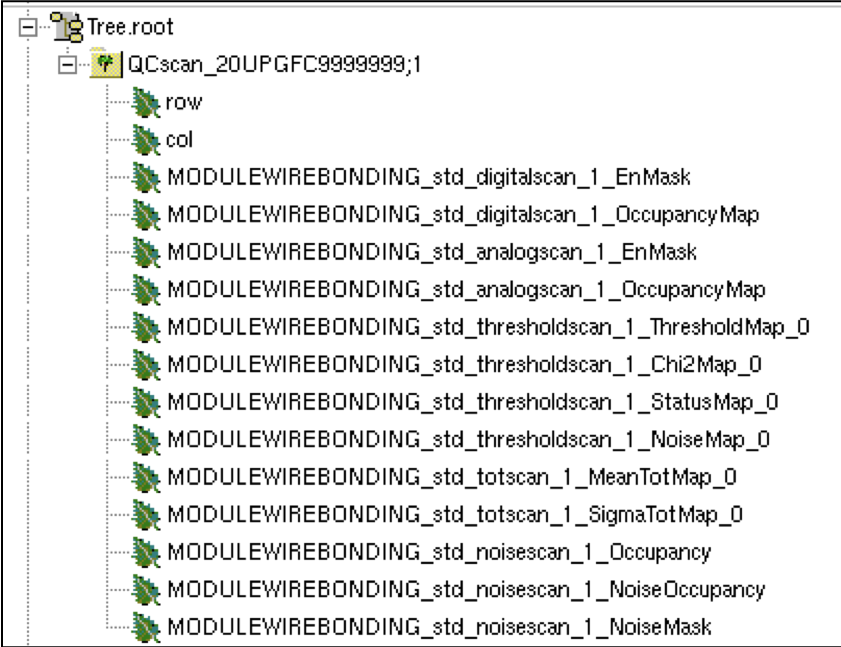
\includegraphics[width=6cm]{analysis_tool_tree_file}
  \end{minipage}
  \begin{minipage}{0.4\hsize}
    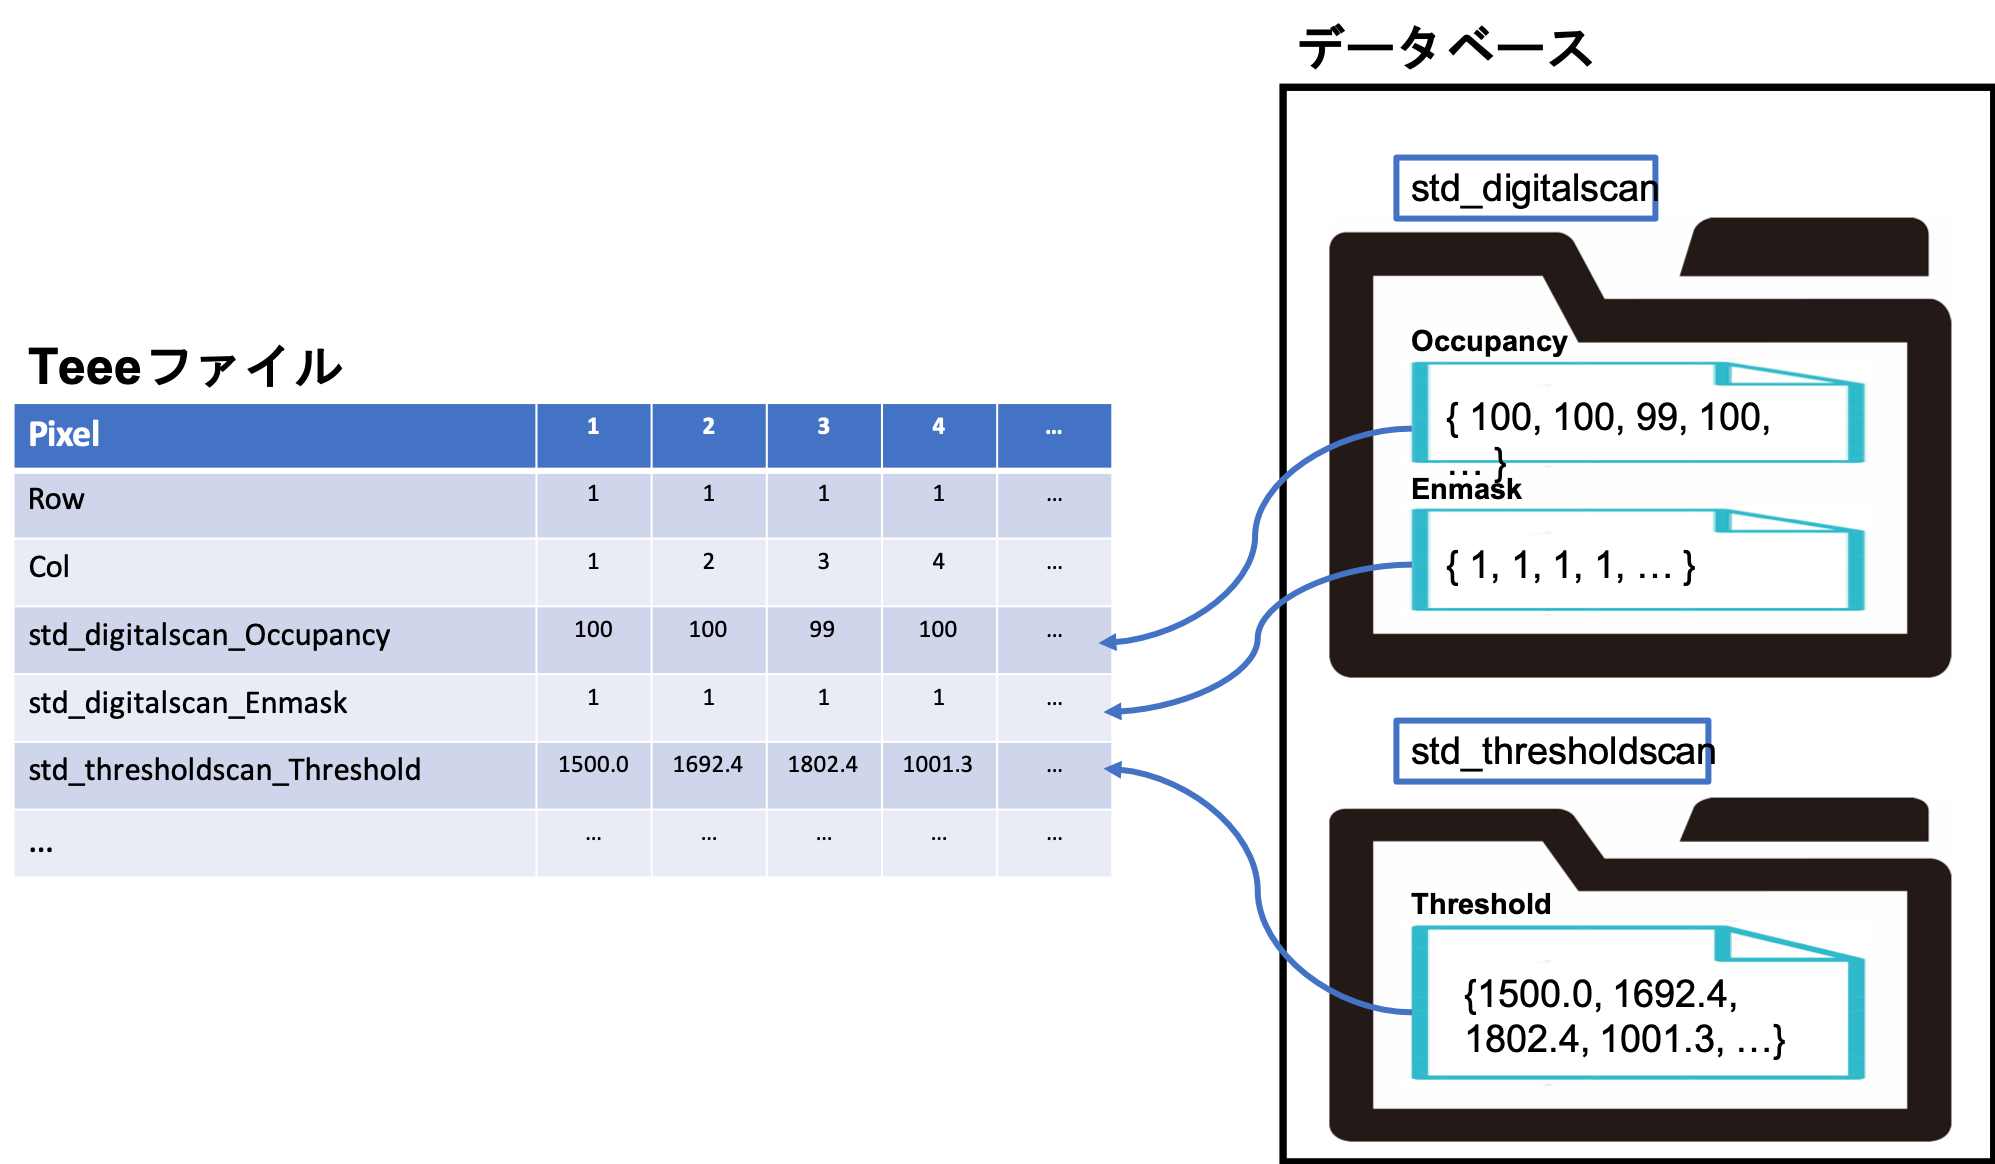
\includegraphics[width=8cm]{analysis_tool_tree_image}
  \end{minipage}
  \caption[Treeファイルとそのデータ保持]{Treeファイルとそのデータ保持}
  \label{analysis_tool_tree}
  \end{center}
\end{figure}

\clearpage
\subsection{ツールの内部構造と処理の流れ}
開発したツールは、主に以下で説明する3つの実行ファイルで構成される。それぞれの役割について説明する。

\begin{description}
  \item[getDataFile.py (Python)]\mbox{}\\ 
    データベースから対象となるデータファイルを取得、キャッシュファイルとしてサーバー上の一時ディレクトリに保存.
  \item[makeTree (C++)]\mbox{}\\ 
    getDataFile.pyを用いて生成されたキャッシュファイルを読み込み、Treeファイルを作成.
  \item[analysis (C++)]\mbox{}\\ 
  作成したTreeファイルを読み込み不良ピクセル解析を実行、結果値やプロットを出力.
\end{description}

処理の流れのイメージを図\ref{analysis_tool_flow}に示す。
データベースとの通信に関してはMongoDBや現システムとの親和性を考慮し、Pythonを使用した。
Treeファイル作成やその後の解析処理のスクリプトは、ROOTを使用の観点からC++を使用した。
またピクセル解析以外の解析に対しても適応可能とするため、Tree作成部と解析処理部は分割している。

\begin{figure}[bpt]\centering
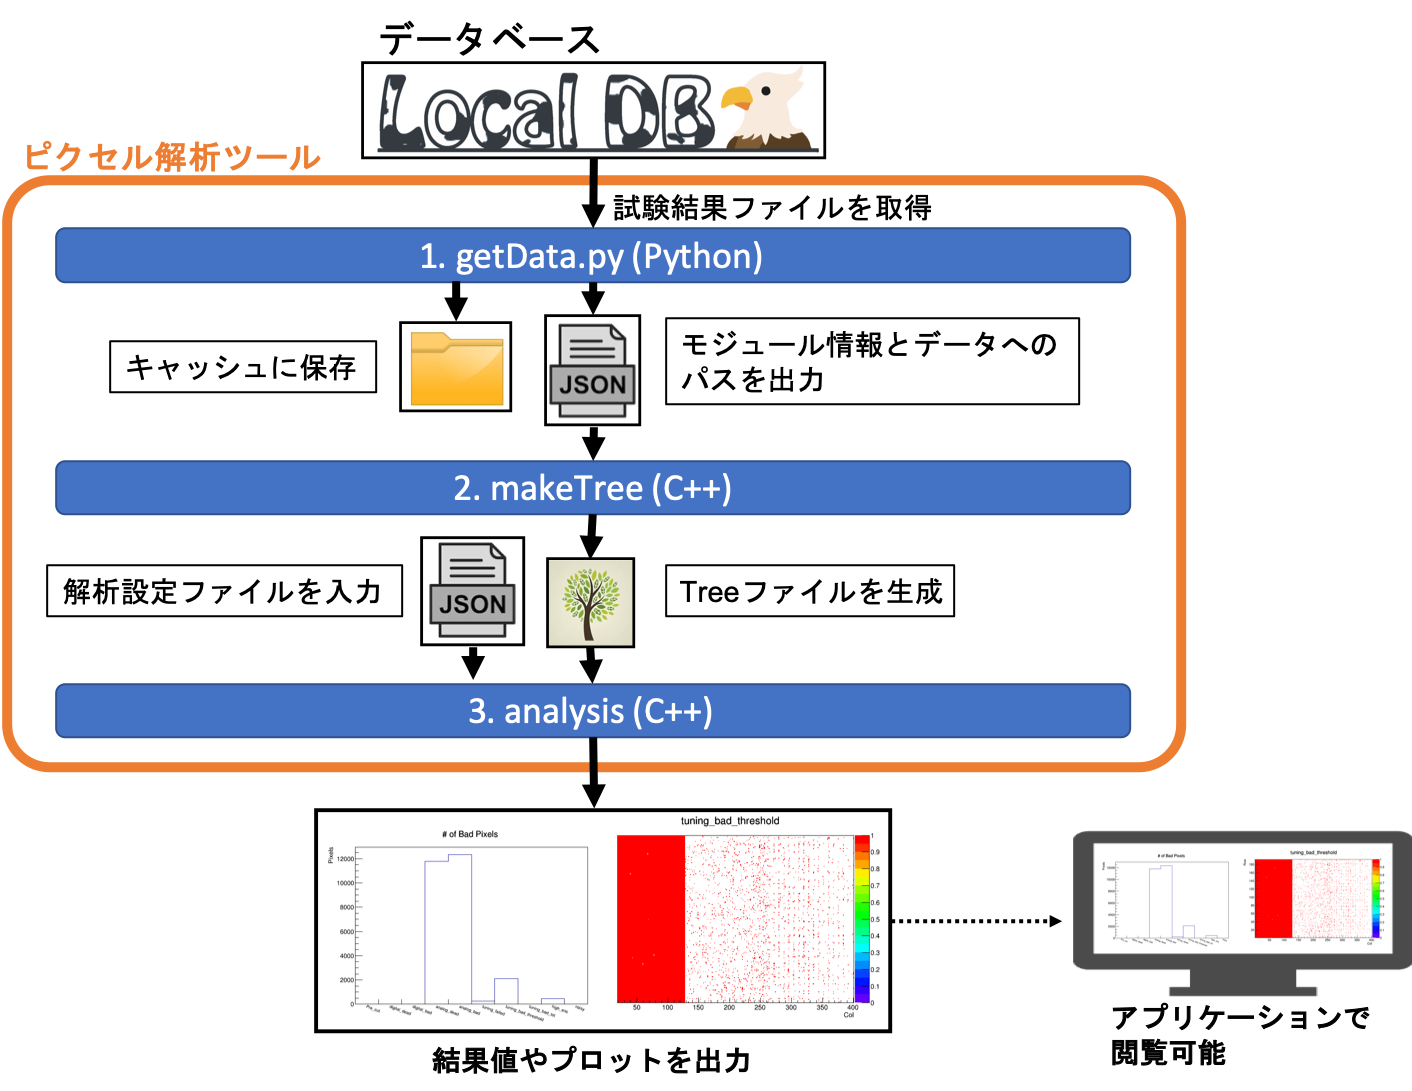
\includegraphics[width=12cm]{analysis_tool_flow}
\caption[ピクセル解析ツールの処理の流れ]{ピクセル解析ツールの処理の流れ}
\label{analysis_tool_flow}
\end{figure}

\clearpage
\section{学内実験室におけるデモンストレーション}

上述したピクセル解析ツールを含む読み出し試験用ソフトウェアの機能確認を目的として、生産時における流れのデモンストレーションを学内実験室で行なった。
その詳細について以下に示す。

\subsection{用いたソフトウェアの概要}

試験で用いたソフトウェアをいかに示す。
また、これらソフトウェアの概要を図\ref{readout_SW_overview}に示す。
\begin{itemize}
  \item YARR(commit:6b3ffe92)
  \item MongoDB(version: v4.2.6)
  \item ローカルDBウェブアプリケーション(tag: ldbtoolv1.4)
  \item 中央データベースとの同期ツール(tag: ldbtoolv1.4)
  \item ピクセル解析ツール(tag: v1.0.2)
  \item 時系列データ用データベース(InfluxDB\cite{5-6}(version: 1.8.0))
    \begin{itemize}
      \item 時系列情報に特化したデータベース。このシステムにおいては温度、電圧などDCS情報を時間情報と共に保存、管理するために用いる。
    \end{itemize}
  \item InfluxDB解析ソフト(Grafana\cite{5-7}(version: 5.1.0))
    \begin{itemize}
      \item InfluxDBに保存された情報の解析、閲覧に用いる。ウェブブラウザー上でDCSデータを閲覧することができる。
    \end{itemize}
  \item 電源操作用ソフト
    \begin{itemize}
      \item 電源を遠隔で操作し、モジュールに電圧を供給する。また電圧、電流値を取得し、InfluxDBにアップロードする。CERNで開発されているPySerial\cite{5-8}(commit:0d14fcdb)を改良し作成した。
    \end{itemize}
  \item 温度読み出し用ソフト
    \begin{itemize}
      \item GPIO通信により取得できるADC値を取得、温度に変換しInfluxDBへアップロードする処理を作成したもの。RaspberryPi上に保存し、処理を実行。
    \end{itemize}
\end{itemize}

\begin{figure}[bpt]\centering
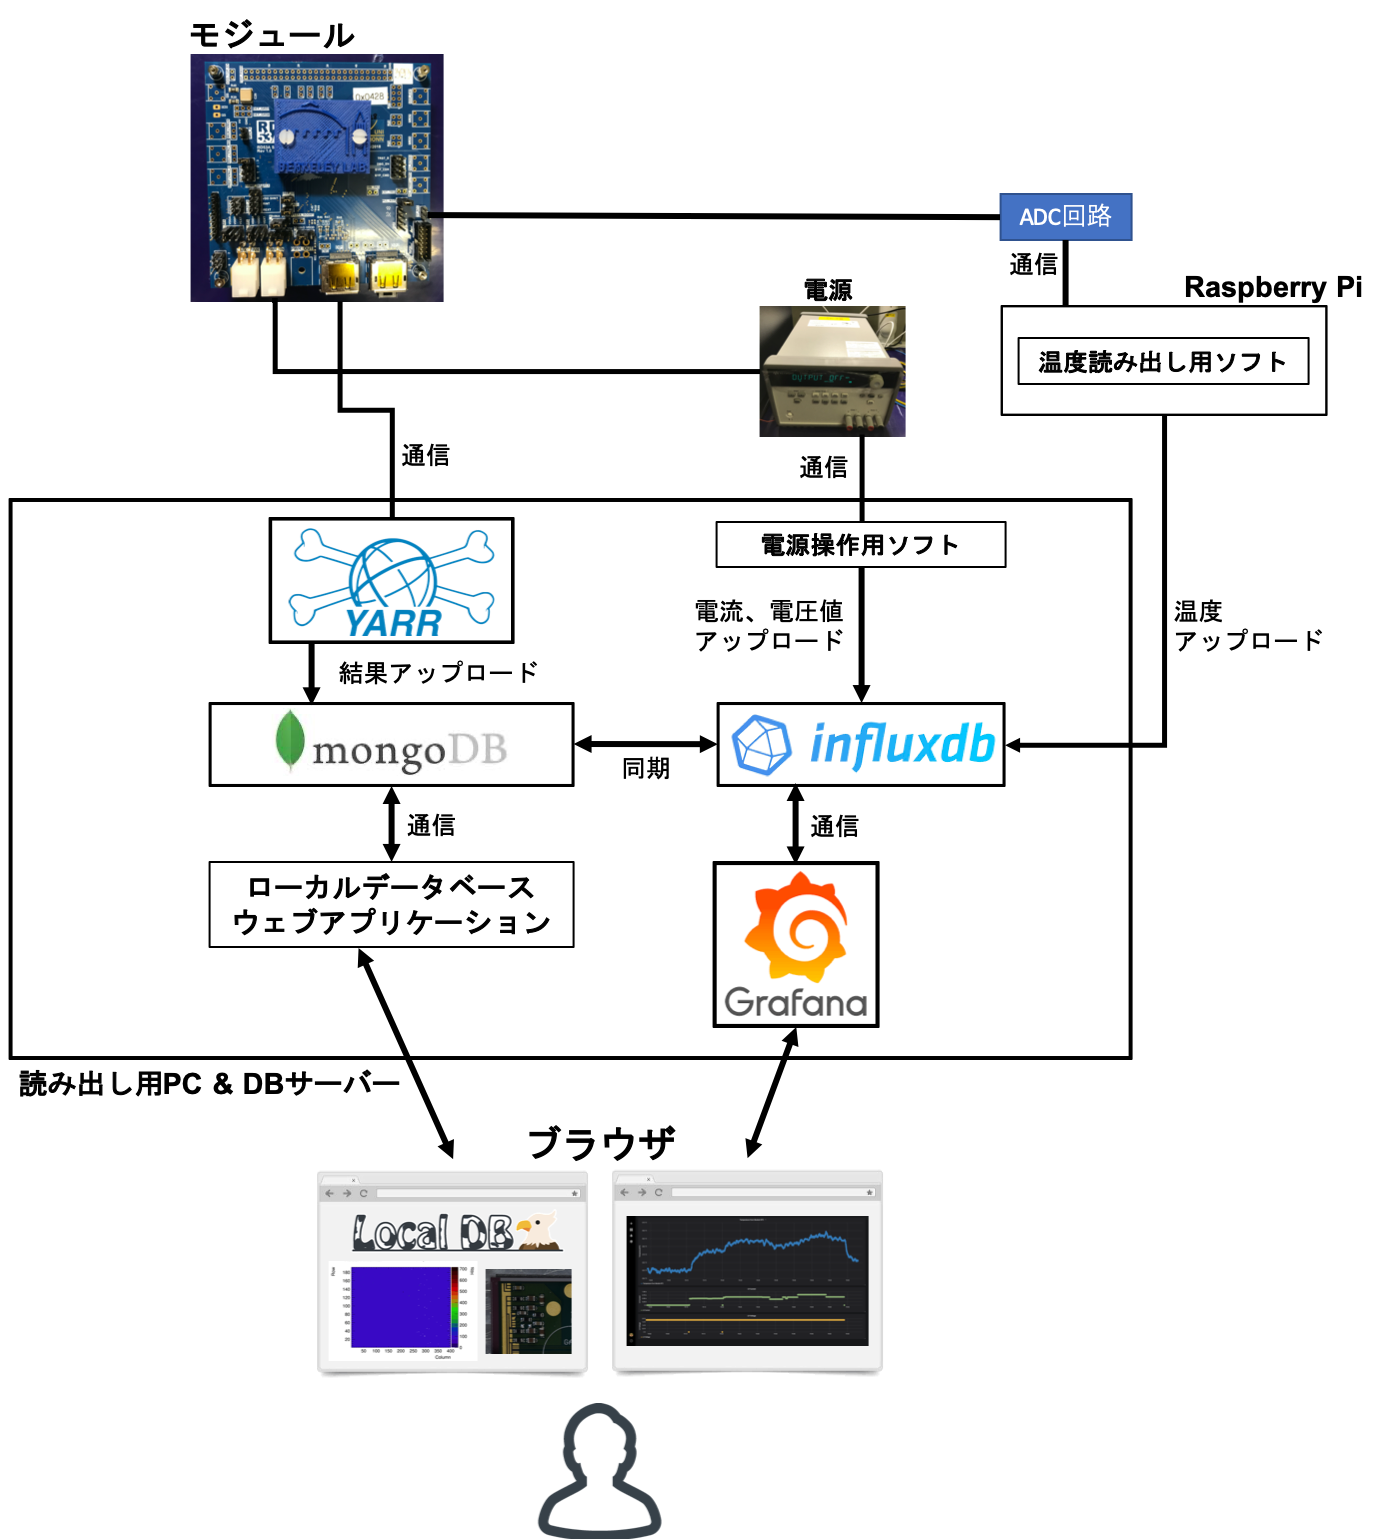
\includegraphics[width=14cm]{readout_SW_overview}
\caption[読み出し試験に用いるソフトウェアの概要]{読み出し試験に用いるソフトウェアの概要}
\label{readout_SW_overview}
\end{figure}

\clearpage
\subsection{用いたハードウェア}
読み出し試験に用いたハードウェアについて、以下に詳細を記す。

\subsubsection{RD53Aシングルモジュール(RD53A Single Chip Card, SCC)}
今回読み出しに使うモジュールとして、研究室で所有しているRD53Aシングルモジュール(RD53A Single Chip Card, SCC)を使用した。
SCCは試験用に作られたFEチップを一枚搭載するモジュールである。また今回使用したものはシリコンセンサーを持たない。
SCCはFEチップ電源端子、データ転送端子をもち、読み出しを行う際はそれぞれ配線をする。
FEチップ付近にはNTCサーミスタを搭載していて、ボード上の端子からその抵抗値を取得することで温度を測定することができる。
図\ref{demo_rd53a_SCC}に写真を示す。

\begin{figure}[h]\centering
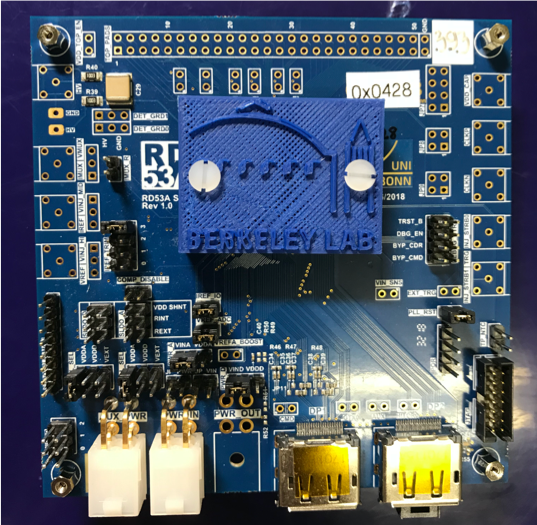
\includegraphics[width=8cm]{rd53a_SCC}
\caption[RD53A]{RD53A}
\label{demo_rd53a_SCC}
\end{figure}

\subsubsection{モジュールサーミスタ温度読み出しシステム}
モジュール付属のサーミスタ、ADC、Raspberry Piを用いた温度読み出しシステムを作成した。
このシステムの中で扱った装置を表\ref{demo_temp_device}に、回路図、実際に配線した様子を図\ref{demo_temp_circit_pic}に示す。
スクリプト上でサーミスタの抵抗値に対応するADC値を温度に変換することで読み出しを行っている。
ADC値はGPIO通信\cite{5-9}により取得している。

\begin{table}[tbp]
\begin{center}
\caption[hoge]{hoge}
\label{demo_temp_device}
  \begin{tabular}{|ll|} \hline
    装置 & 機種 \\ \hline
    10$\rm{k\Omega}$抵抗 & - \\
    ADC & MCP3002\cite{5-3} \\  
    RaspberryPi &  Raspberry Pi 3 Model B Plus Rev 1.3\cite{5-4} \\ \hline 
  \end{tabular}
\end{center}
\end{table}

\begin{figure}[h]\centering
  \begin{minipage}{0.5\hsize}
    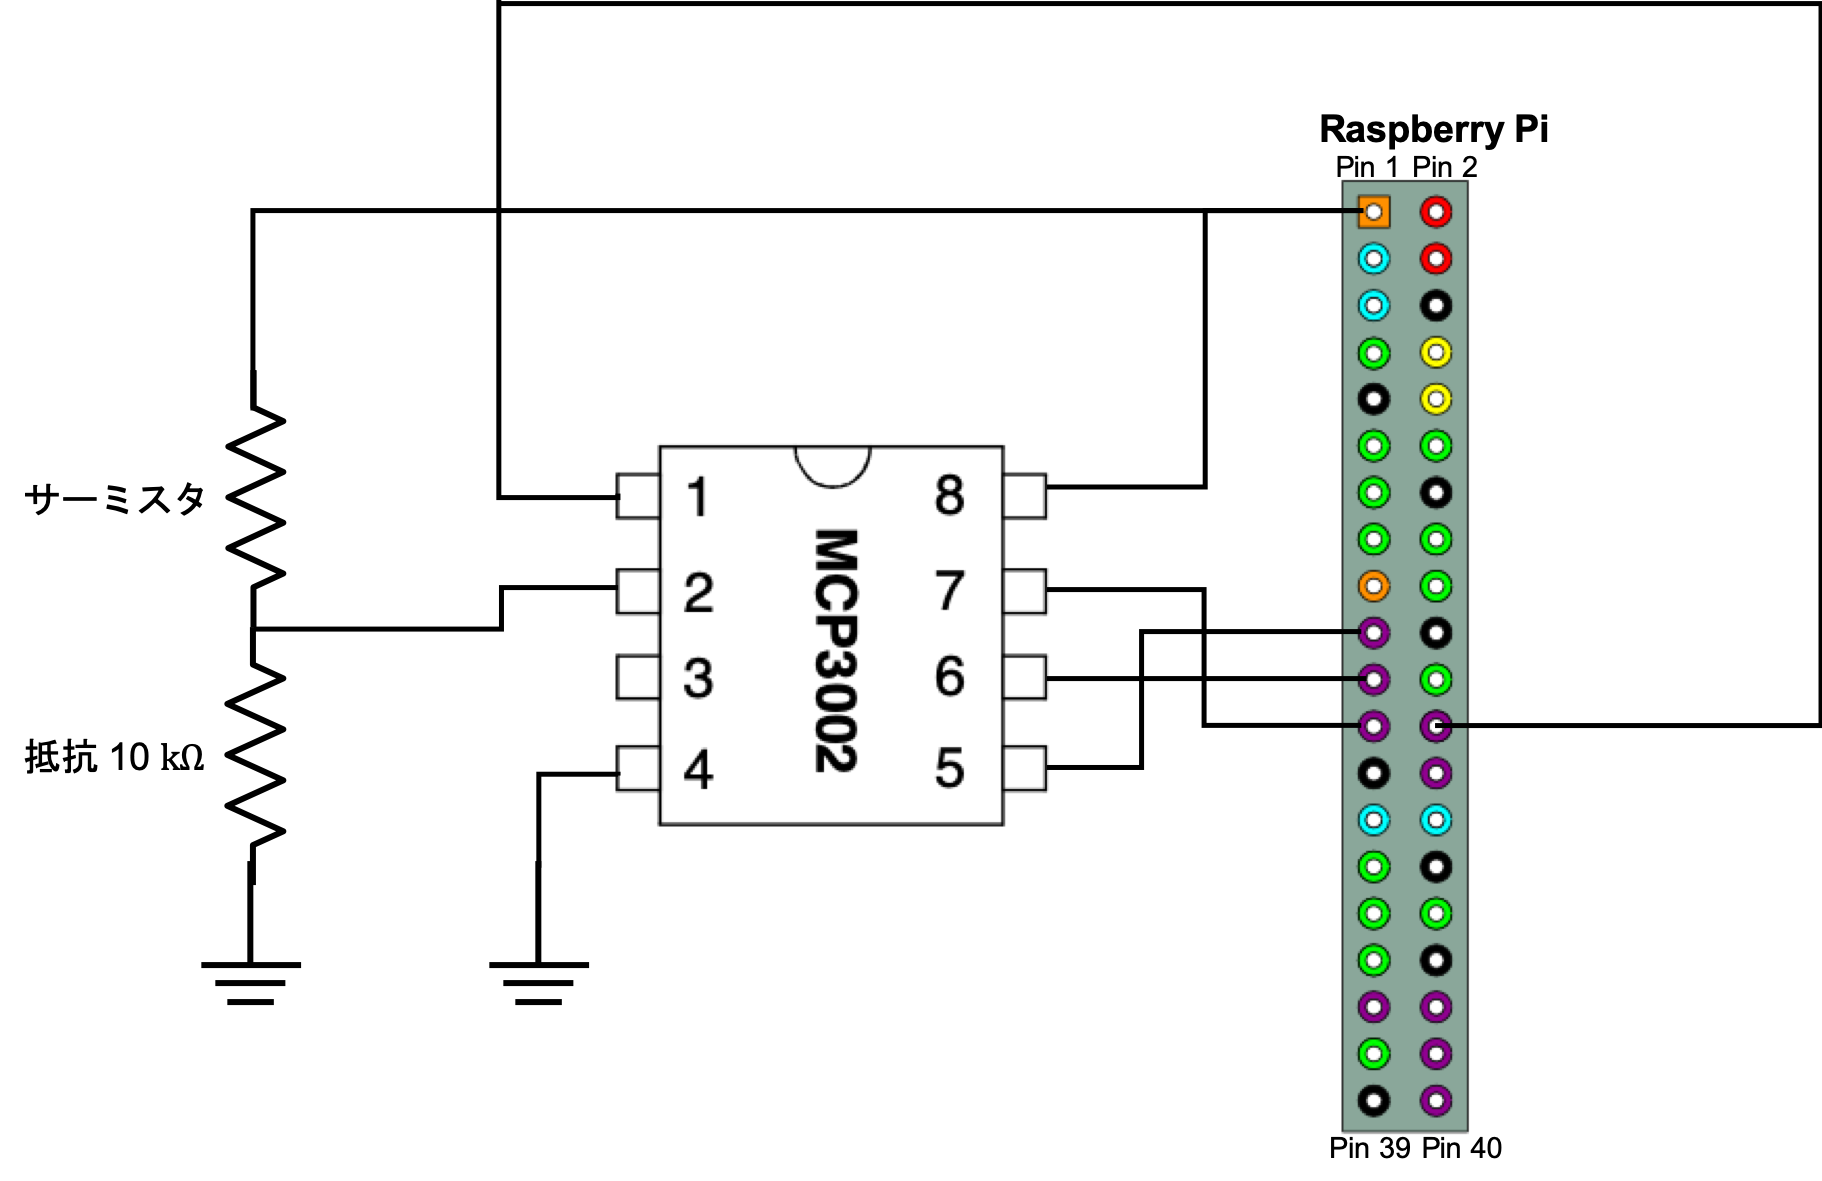
\includegraphics[width=7cm]{temp_circit}
  \end{minipage}
  \begin{minipage}{0.4\hsize}
    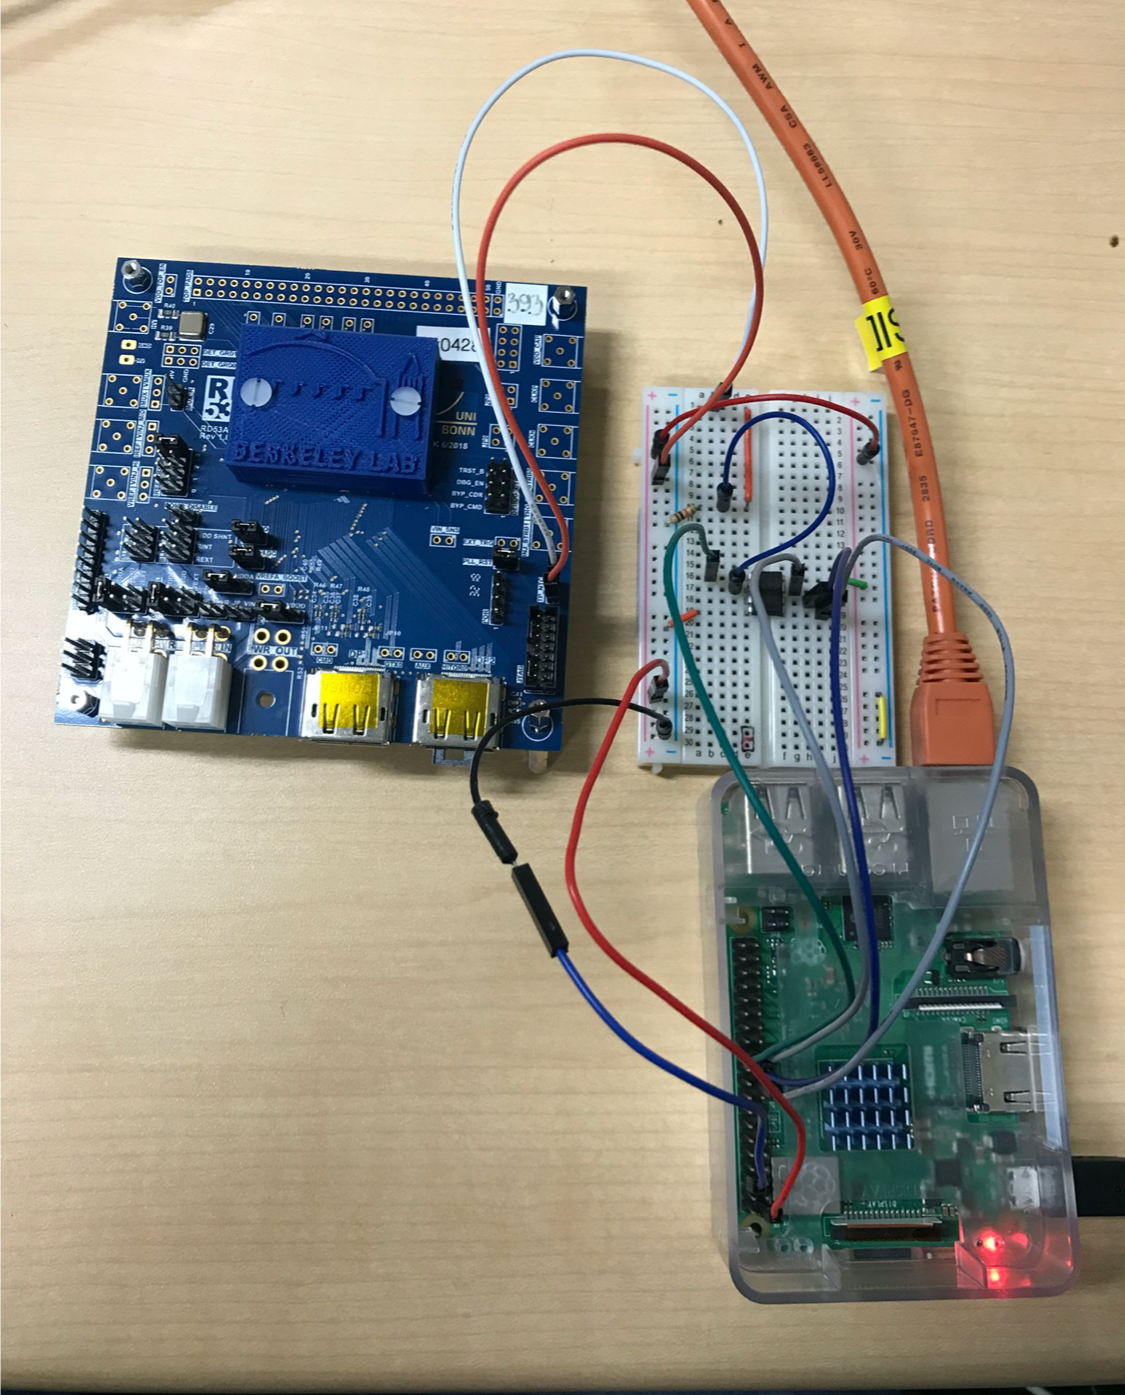
\includegraphics[width=5cm]{temp_circit_pic}
  \end{minipage}
\caption[モジュール付属サーミスタを用いた温度読み出し回路]{モジュール付属サーミスタを用いた温度読み出し回路}
\label{demo_temp_circit_pic}
\end{figure}

\subsubsection{電源}
モジュールの電圧供給にKEYSIGHTのE3646A 60Wデュアル出力電源\cite{5-1}(図\ref{demo_power_supply})を用いた。
\begin{figure}[h]\centering
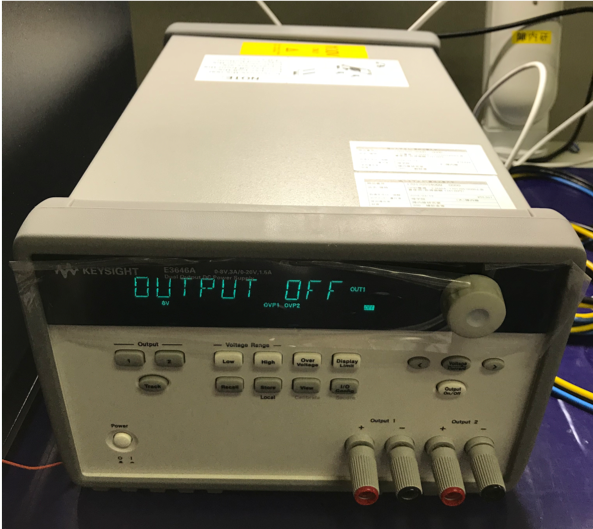
\includegraphics[width=6cm]{power_supply}
\caption[電源]{電源}
\label{demo_power_supply}
\end{figure}

\subsubsection{FPGAボード}
FPGAボードにXpressK7\cite{5-2}(図\ref{demo_fpga_board})を用いた。

\subsubsection{FMC-DisplayPort変換カード}
今回使用したFMC-DisplayPort変換カード(Ohio Card)を図\ref{demo_ohio}に示す。

\begin{figure}[htbp]
 \begin{minipage}{0.5\hsize}
  \begin{center}
   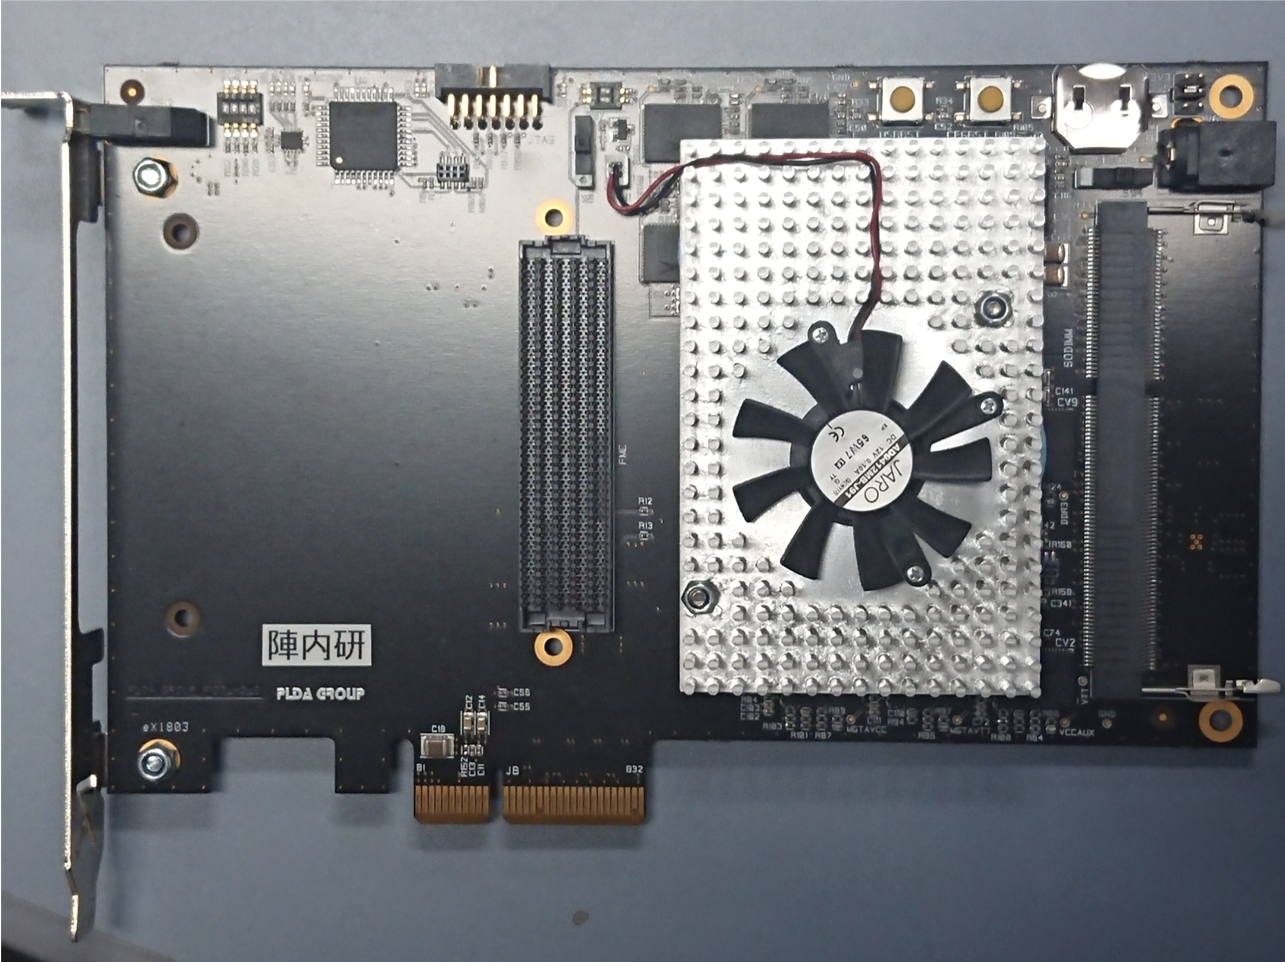
\includegraphics[width=60mm]{fpga_board}
  \end{center}
  \caption[FPGAボード]{FPGAボード}
  \label{demo_fpga_board}
 \end{minipage}
 \begin{minipage}{0.5\hsize}
  \begin{center}
   
\includegraphics[width=60mm]{figure}
  \end{center}
  \caption[オハイオ]{オハイオ}
  \label{demo_ohio}
 \end{minipage}
\end{figure}

\subsubsection{PC}
今回用いたPCの性能を表\ref{daq_machine_spec}に示す。
\begin{table}[tbp]
\begin{center}
\caption[]{}
\label{daq_machine_spec}
\scalebox{0.9}{
  \begin{tabular}{|llll|l|l|} \hline
    CPU & & & & Memory & Disk \\
    Type & Core & Thread & Clock speed[GHz]& [GB] & [GB] \\ \hline 
    Intel(R) Core(TM) i7-8700K CPU & 6 & 12 & 3.7 & 16.18 & 214\\ \hline
  \end{tabular}
}
\end{center}
\end{table}

\subsubsection{セットアップ}
読み出し試験に用いるハードウェアのセットアップを概要を図\ref{readout_setup_overview}に示す。

\begin{figure}[bpt]\centering
  \begin{minipage}{0.5\hsize}
    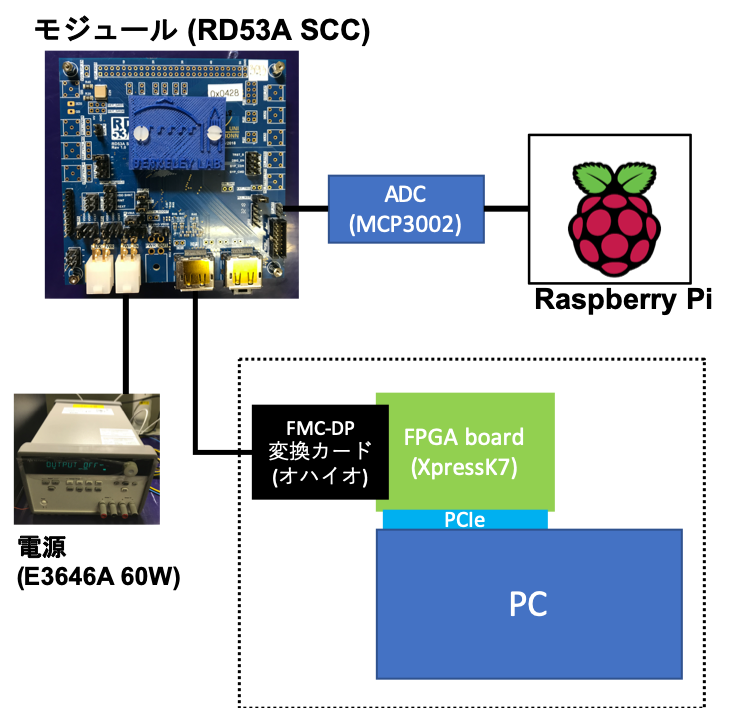
\includegraphics[width=7cm]{HW_setup}
  \end{minipage}
  \begin{minipage}{0.4\hsize}
    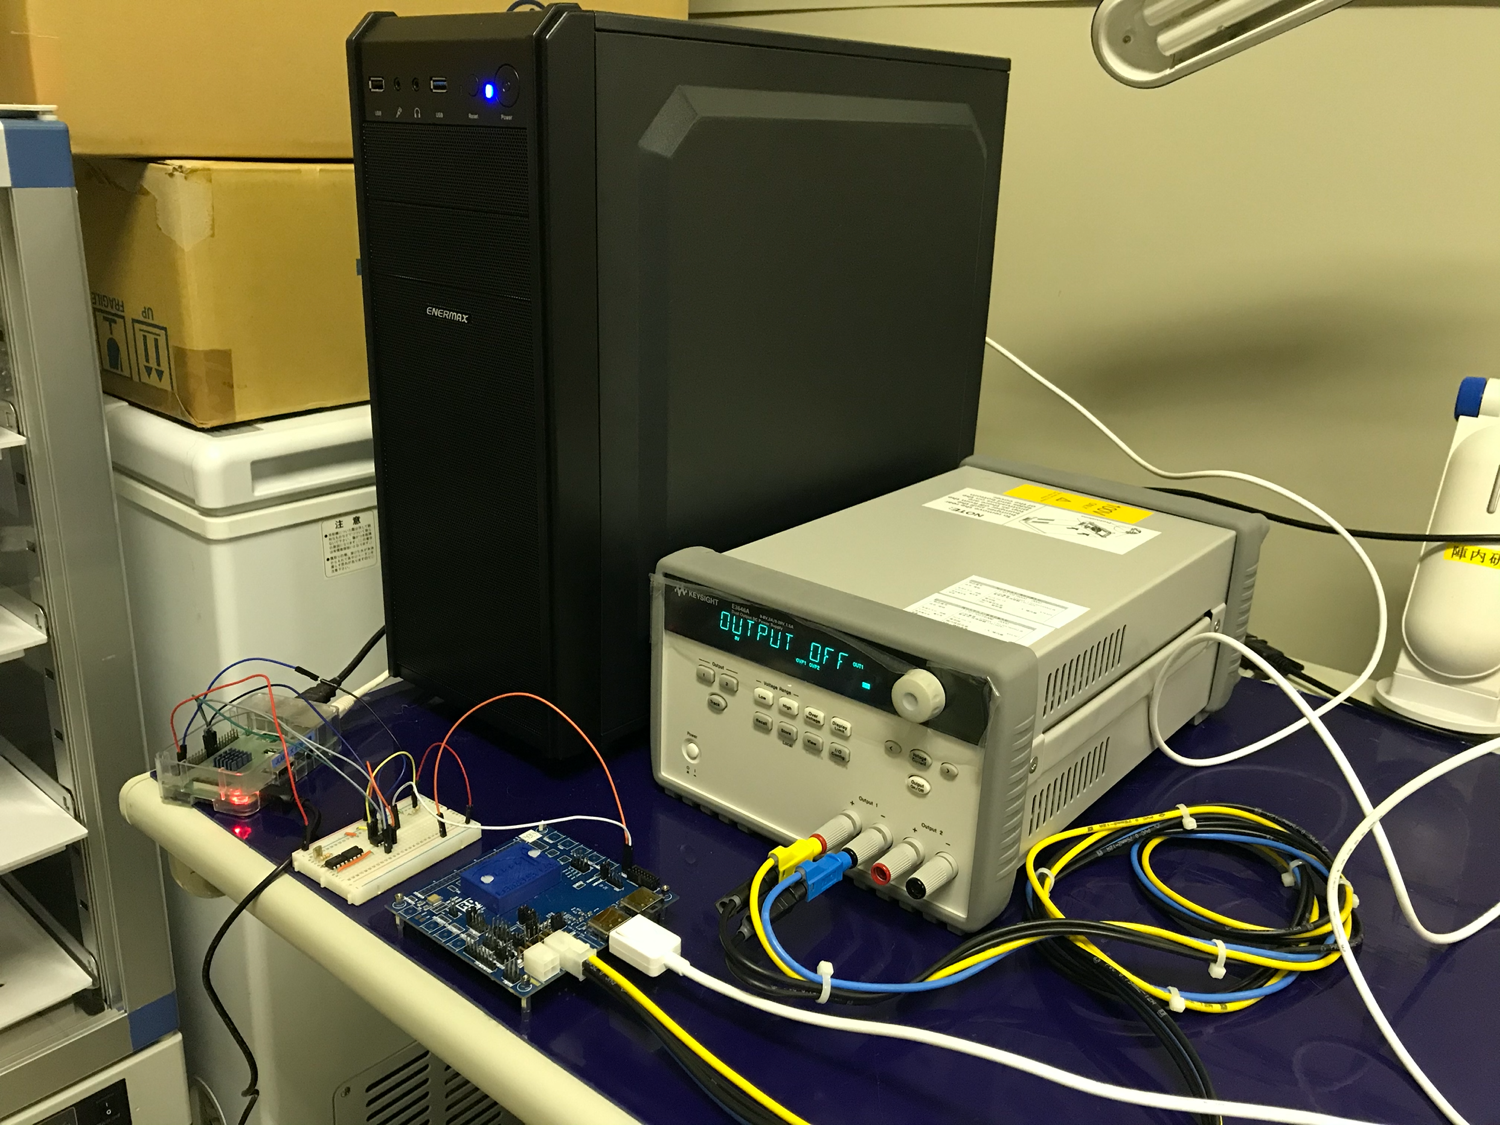
\includegraphics[width=6.5cm]{HW_setup_pic}
  \end{minipage}
\caption[ハードウェアセットアップの概要]{ハードウェアセットアップの概要}
\label{readout_setup_overview}
\end{figure}


%%%%%%%%%%%%%%%%%%%%%%%%%%%%%%%%%%%%%%%%%%%%%%%%%
%%%%%%%%%%%%%%%%%%%%%%%%%%%%%%%%%%%%%%%%%%%%%%%%%
%%%%%%%%%%%%%%%%%%%%%%%%%%%%%%%%%%%%%%%%%%%%%%%%%
\clearpage
\subsection{デモンストレーションの流れ}
デモンストレーションで扱うモジュールとして以下のモジュール、FEチップを中央データベースに登録した。
\begin{description}
  \item[モジュールID] 20UPGR00000001
  \item[FEチップID] 20UPGFC9999999
\end{description}
今回のデモンストレーションではこれらのIDを用いて試験結果の紐付け等のデータベース操作を行う。

確認した機能を行った流れの順に以下に示す。
\begin{enumerate}
  \item 中央データベースからモジュール情報のダウンロード.
  \item 読み出し試験実施、結果をローカルデータベースに保存.
  \item DCS情報の取得、監視.
  \item 試験結果検索.
  \item 試験結果閲覧.
  \item 結果選択とピクセル解析機能.
  \item 中央データベースへ試験結果のアップロード
\end{enumerate}

\subsection{機能確認}
読み出し試験を通して、各ソフトウェア機能が正しく動くことを確認した。
詳細を以下に記す。

\subsubsection{中央データベースからモジュール情報のダウンロード}
ダウンロードし、ウェブアプリケーションで確認した。
確認した画面を図\ref{demo_download_SCC}に示す。
今回行った試験結果はこのモジュールに紐つける形でローカルデータベースに保存される。

\begin{figure}[bpt]\centering
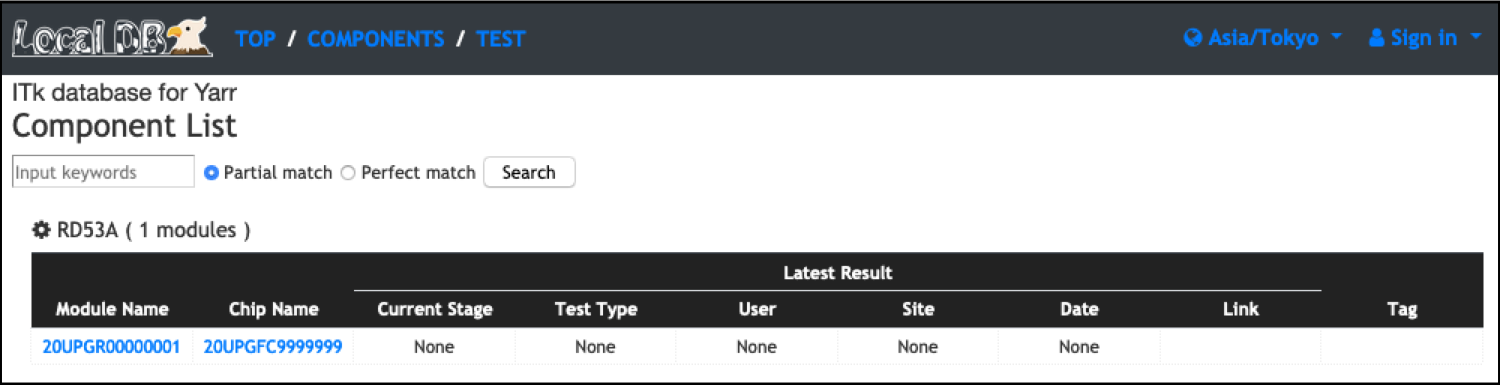
\includegraphics[width=14cm]{demo_download_SCC}
\caption[ダウンロードしたモジュールID確認画面]{ダウンロードしたモジュールID確認画面}
\label{demo_download_SCC}
\end{figure}

%%%%%%%%%%%%%%%%%%%%%%%%%%%%%%%%%%%%%%%%%%%%%%%%%
%%%%%%%%%%%%%%%%%%%%%%%%%%%%%%%%%%%%%%%%%%%%%%%%%

\clearpage
\subsubsection{読み出し試験実施}
以下の流れに沿って読み出しを行ない、結果をローカルデータベースに保存した。
\begin{enumerate}
  \item デジタル回路読み出し(\texttt{std$\_$digitalscan})
  \item アナログ回路読み出し(\texttt{std$\_$analogscan})
  \item 調整前Threshold測定(\texttt{std$\_$thresholdscan})
  \item Threshold調整
  \item ToT調整
  \item Threshold再調整
  \item 調整後Threshold測定
  \item ToT測定(\texttt{std$\_$totscan})
  \item ノイズ測定(\texttt{std$\_$noisescan})
\end{enumerate}

また読み出し試験を通してDCS情報はInfluxDBを用いて監視し、試験結果と同様にローカルデータベースに保存した。

%%%%%%%%%%%%%%%%%%%%%%%%%%%%%%%%%%%%%%%%%%%%%%%%%
%%%%%%%%%%%%%%%%%%%%%%%%%%%%%%%%%%%%%%%%%%%%%%%%%
\subsubsection{DCS情報の監視}
読み出し試験は、DCS情報を監視しながら行った。
それぞれの値は対応するソフトウェアを用いてInfluxDBにアップロードした。
その値をGrafanaを使って監視をした。その様子を図\ref{demo_monitor_dcs}に示す。

\begin{figure}[bpt]\centering
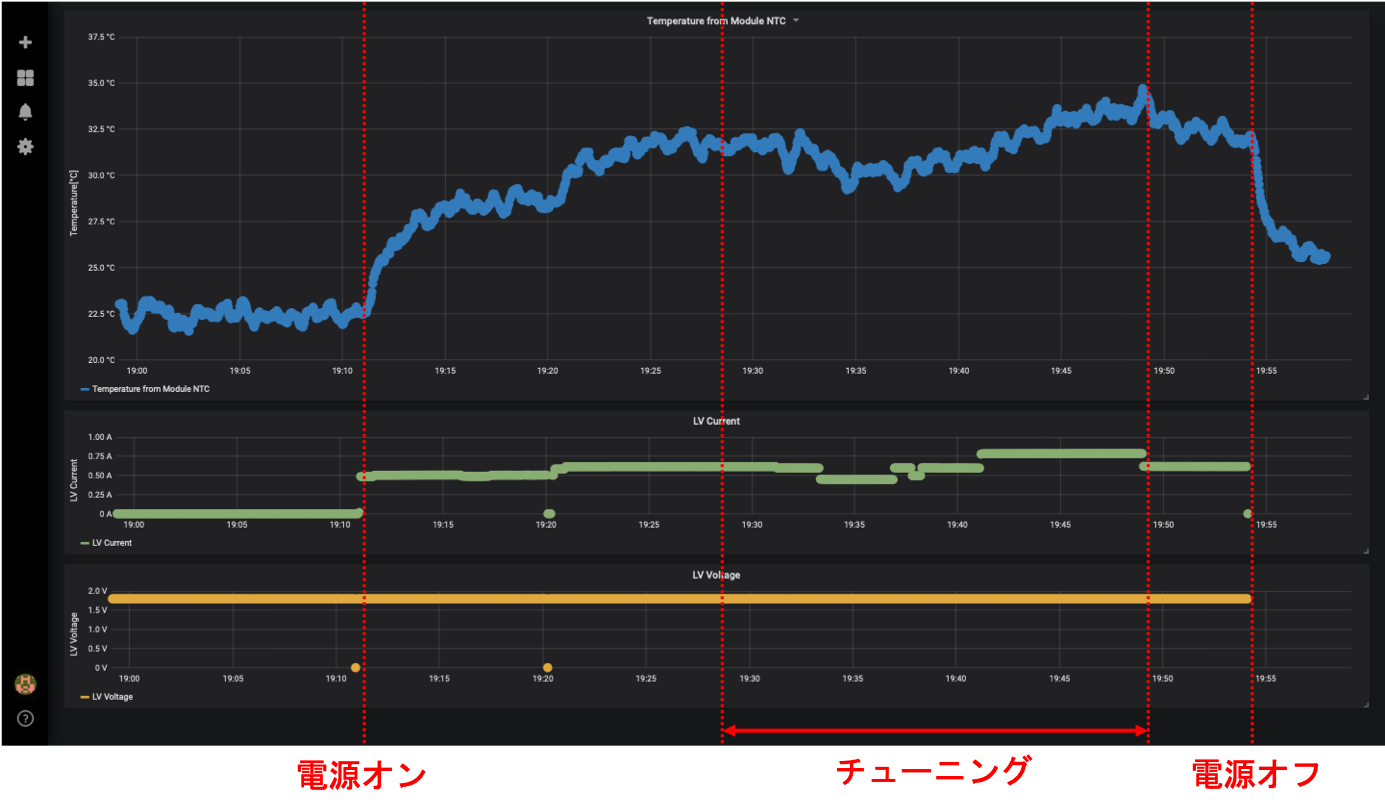
\includegraphics[width=12cm]{demo_monitor_dcs}
\caption[DCSのモニタリング]{DCSのモニタリング}
\label{demo_monitor_dcs}
\end{figure}

%%%%%%%%%%%%%%%%%%%%%%%%%%%%%%%%%%%%%%%%%%%%%%%%%
%%%%%%%%%%%%%%%%%%%%%%%%%%%%%%%%%%%%%%%%%%%%%%%%%
\clearpage
\subsubsection{検索機能の確認}

検索機能の確認を行った。
\begin{figure}[bpt]\centering
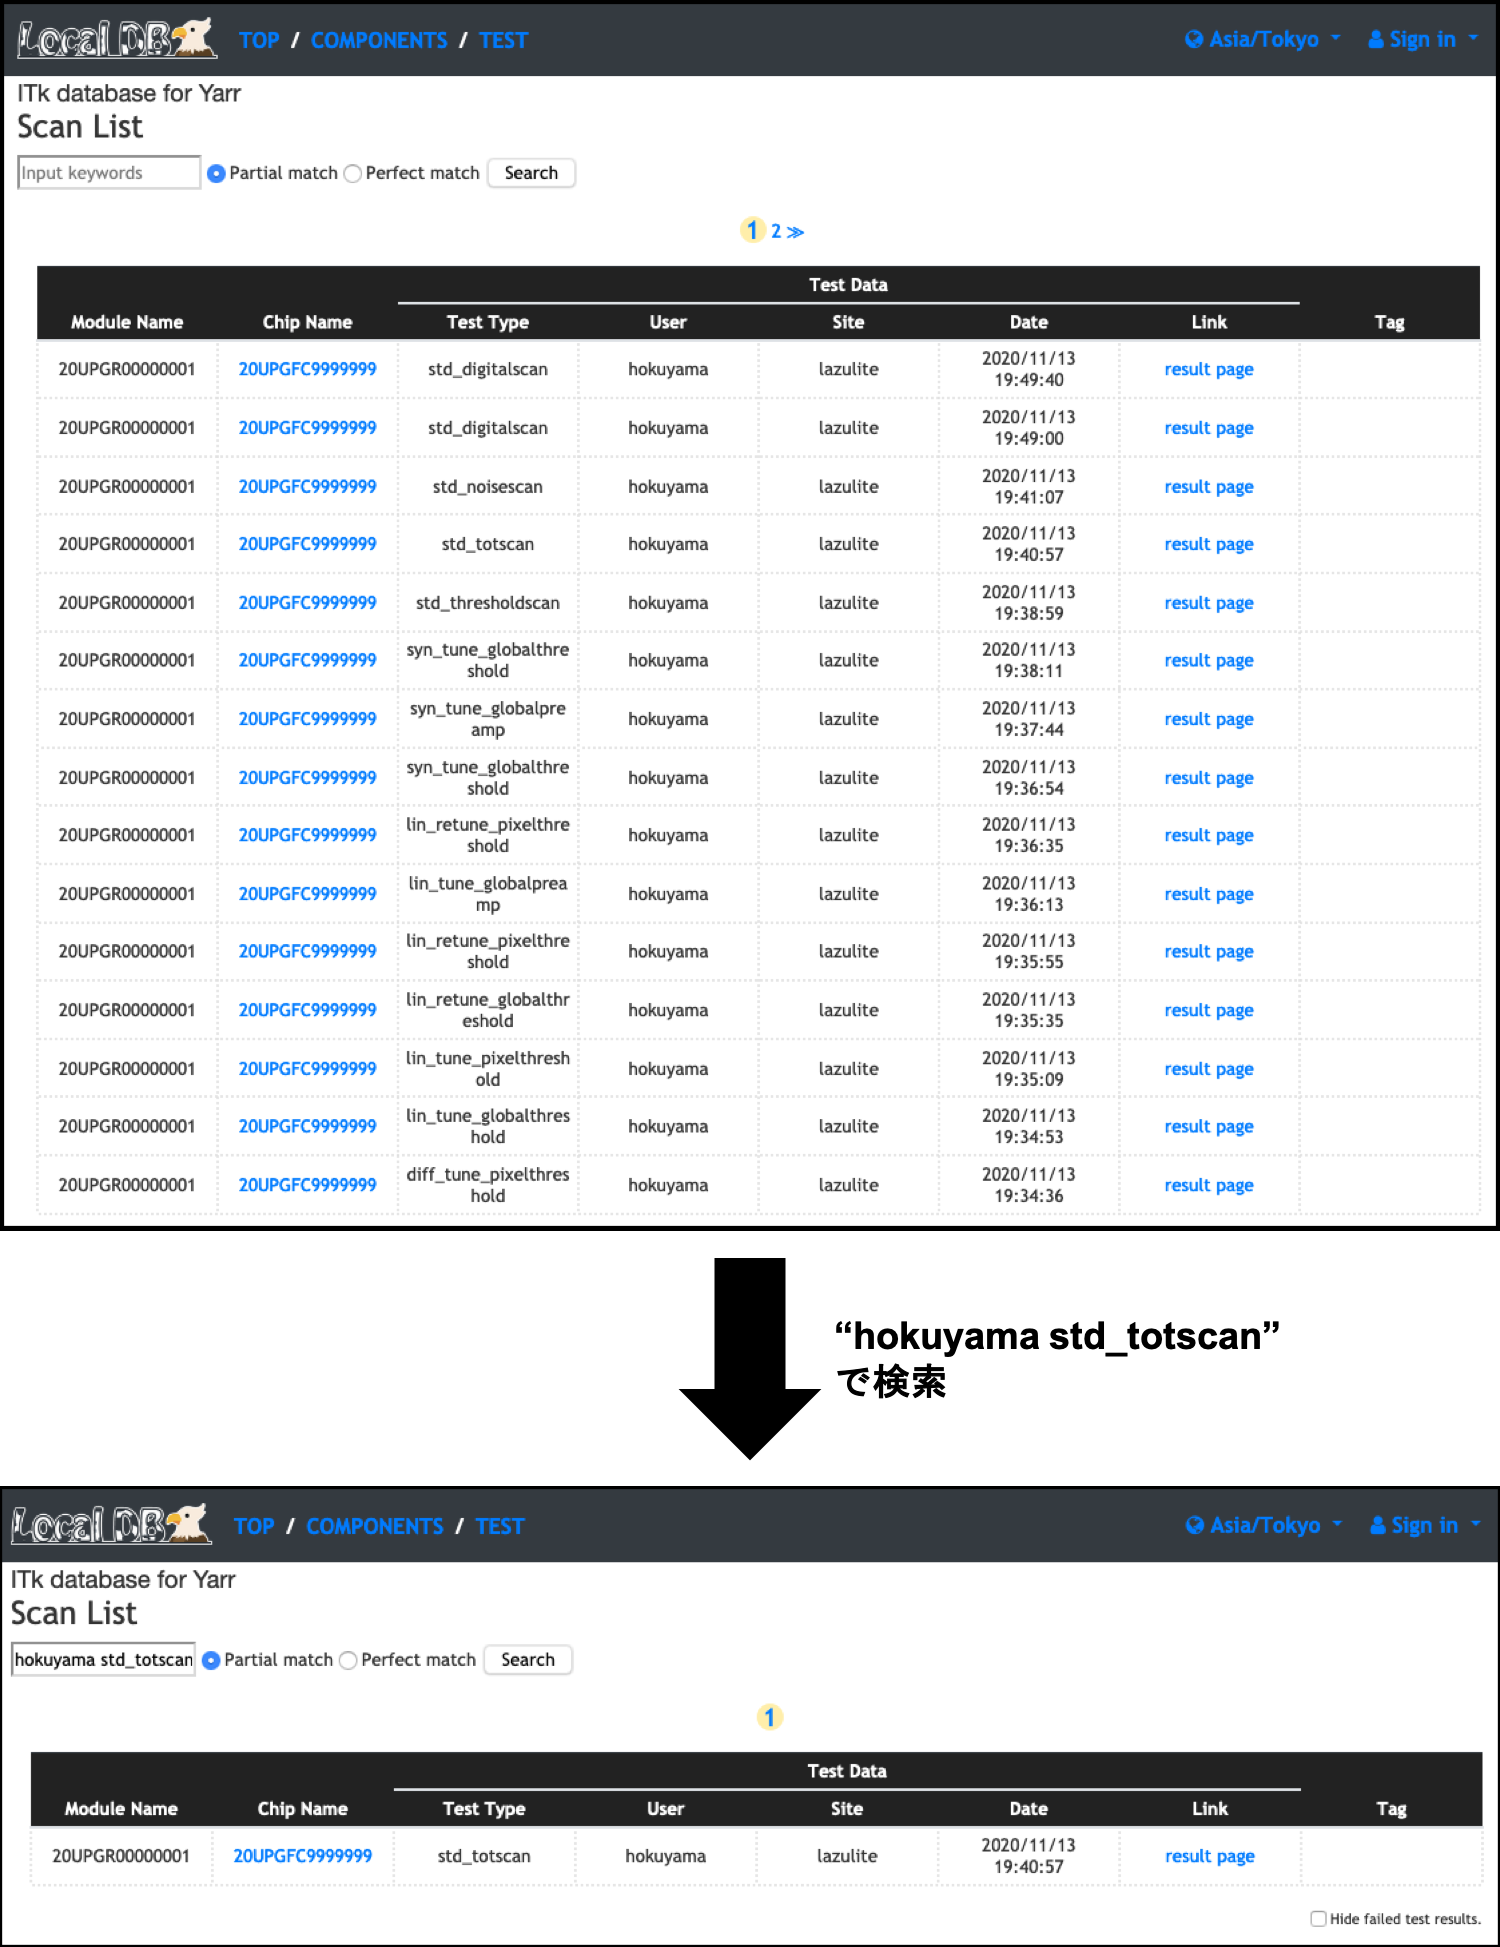
\includegraphics[width=12cm]{demo_search_function}
\caption[検索機能の確認]{検索機能の確認}
\label{demo_search_function}
\end{figure}

%%%%%%%%%%%%%%%%%%%%%%%%%%%%%%%%%%%%%%%%%%%%%%%%%
%%%%%%%%%%%%%%%%%%%%%%%%%%%%%%%%%%%%%%%%%%%%%%%%%
\clearpage
\subsubsection{試験結果の閲覧}
ウェブアプリケーションを用いて、試験結果を閲覧した。その様子を図\ref{demo_view_result}に示す。
\begin{figure}[bpt]\centering
  \begin{minipage}{0.4\hsize}
    \begin{center}
    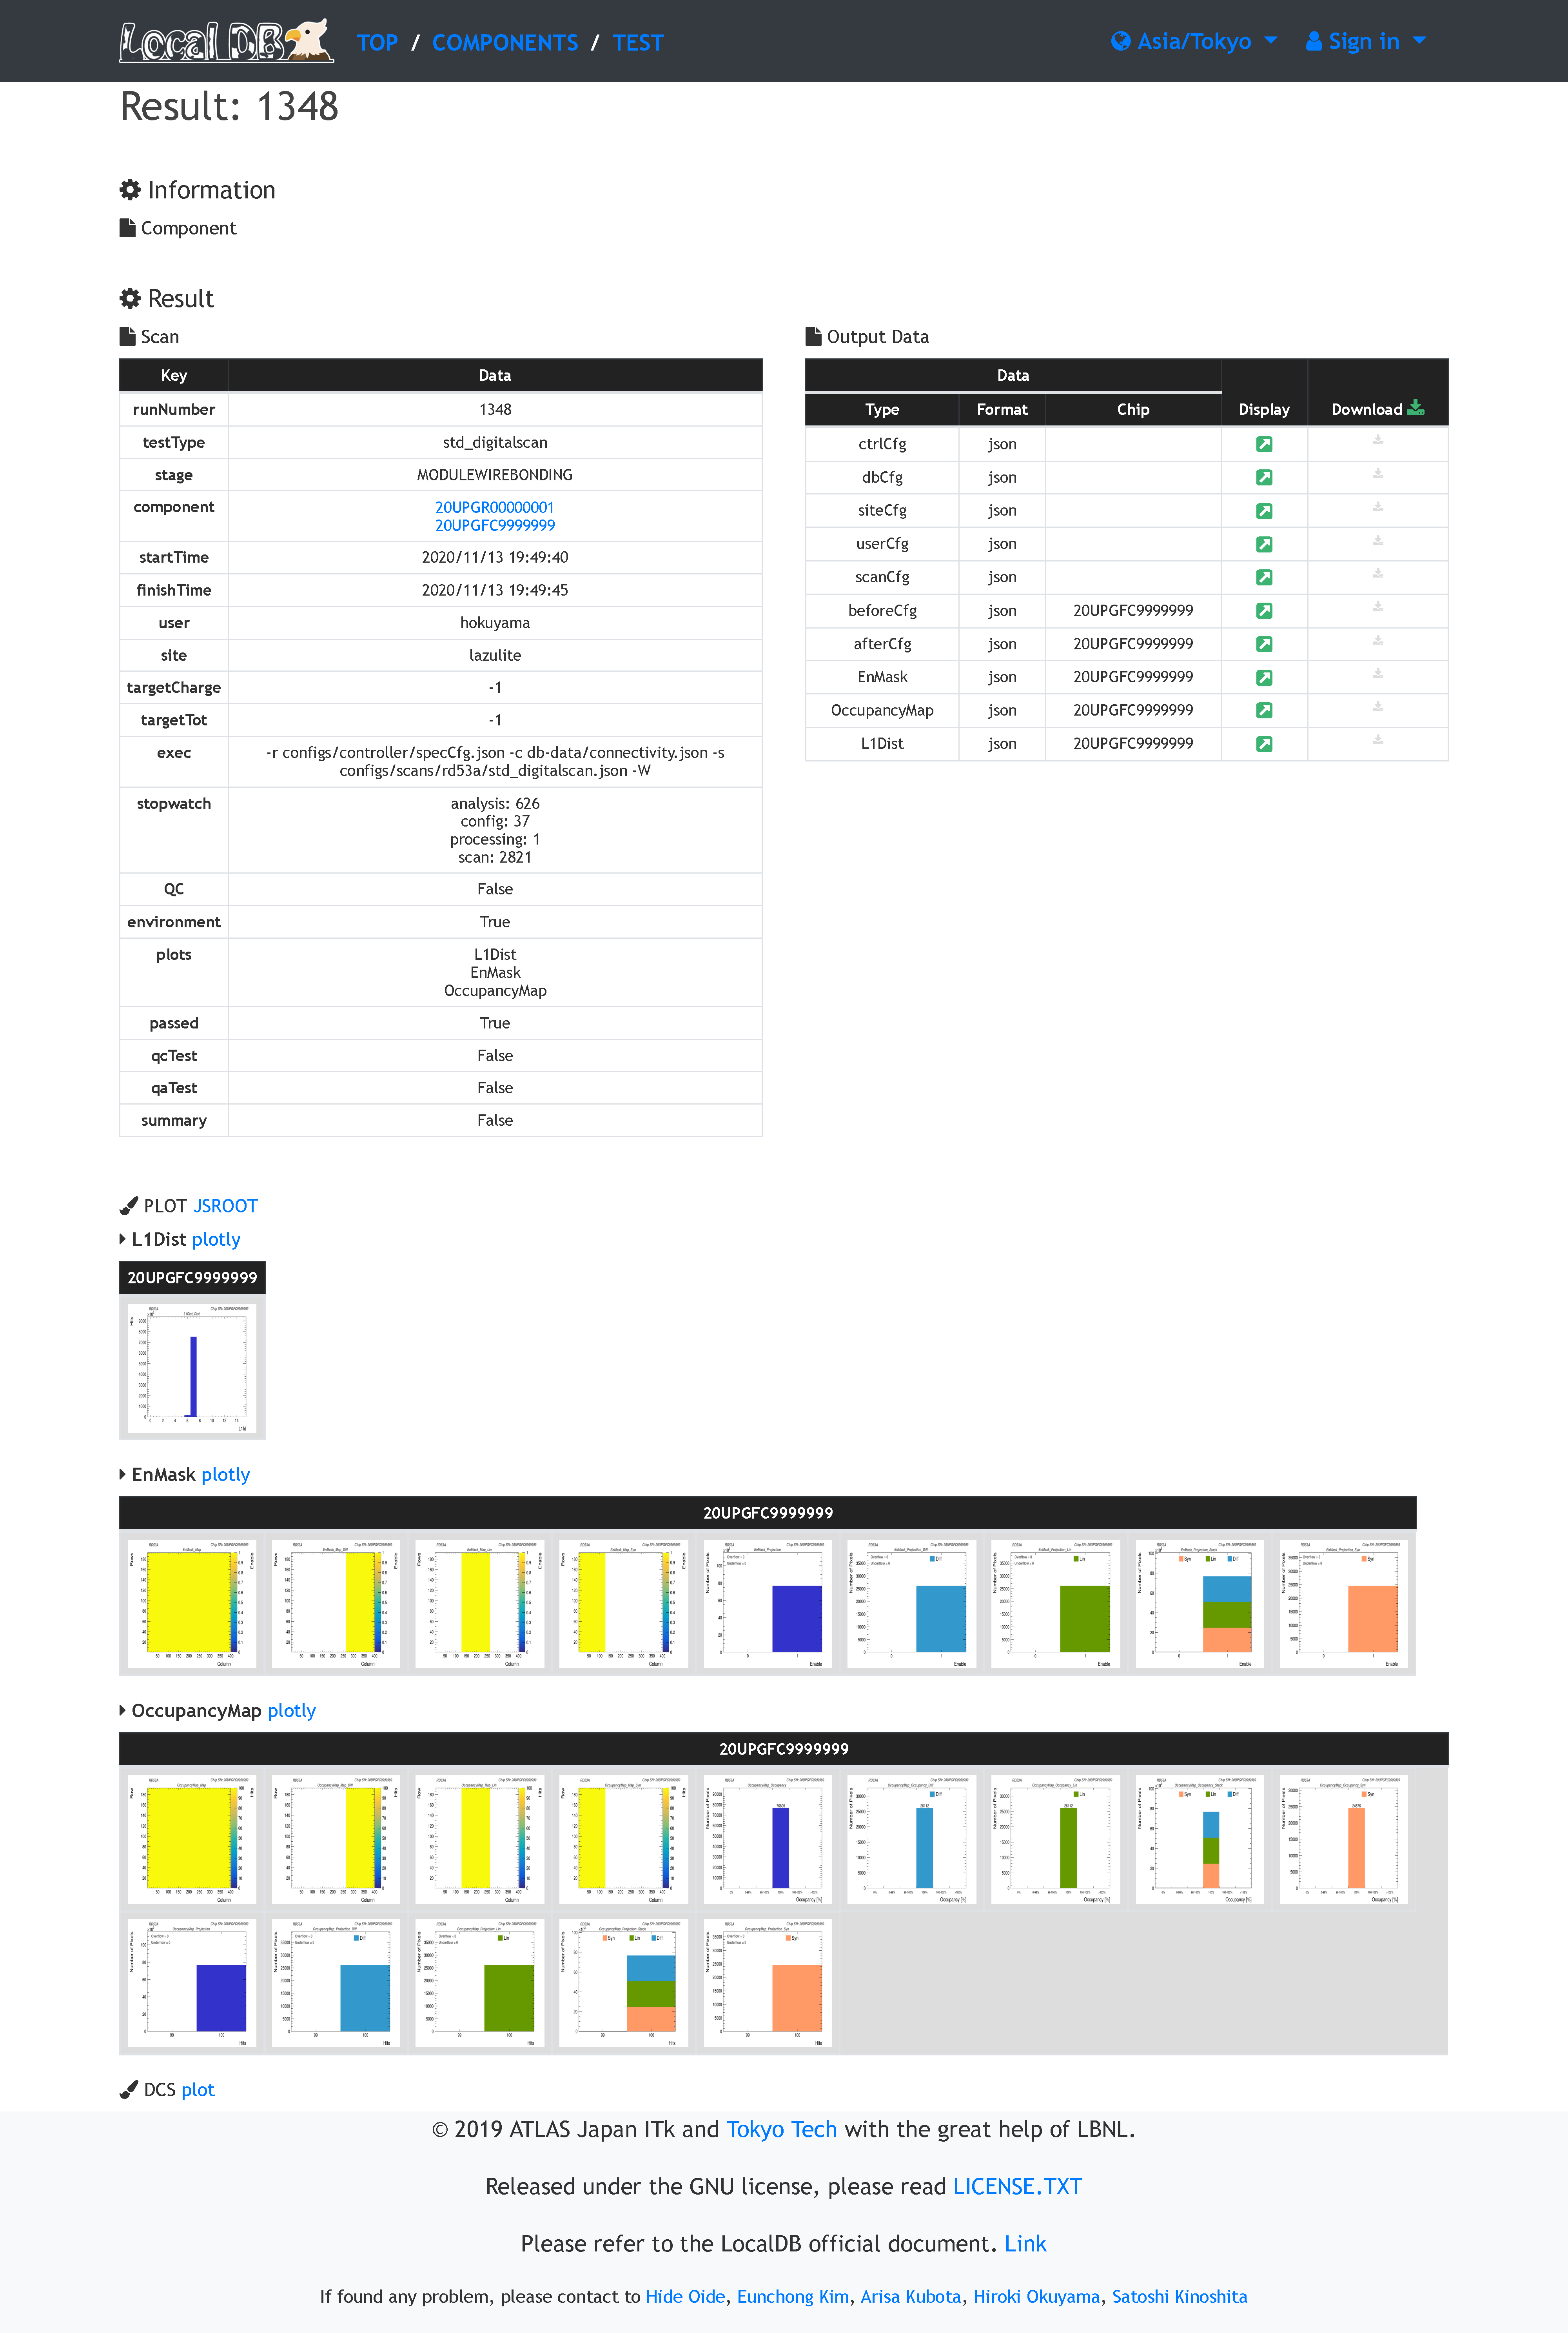
\includegraphics[width=60mm]{demo_view_scan_result}
    \end{center}
  \end{minipage}
  \begin{minipage}{0.4\hsize}
    \begin{center}
    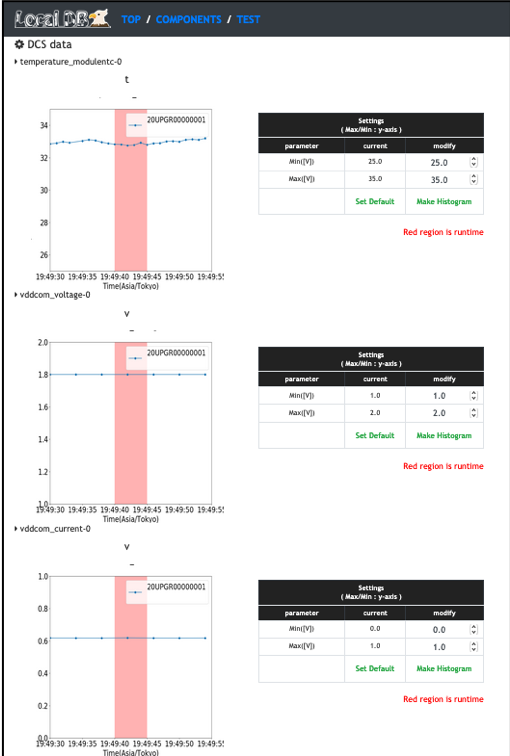
\includegraphics[width=65mm]{demo_view_dcs}
    \end{center}
  \end{minipage}
  \caption[試験結果の閲覧]{試験結果の閲覧}
  \label{demo_view_result}
\end{figure}


%%%%%%%%%%%%%%%%%%%%%%%%%%%%%%%%%%%%%%%%%%%%%%%%%
%%%%%%%%%%%%%%%%%%%%%%%%%%%%%%%%%%%%%%%%%%%%%%%%%
\clearpage
\subsubsection{結果選択とピクセル解析}
読み出し結果を選択し、ピクセル解析を行なった。
結果選択画面を図\ref{demo_select_scans}に示す。

\begin{figure}[bpt]\centering
  \begin{center}
    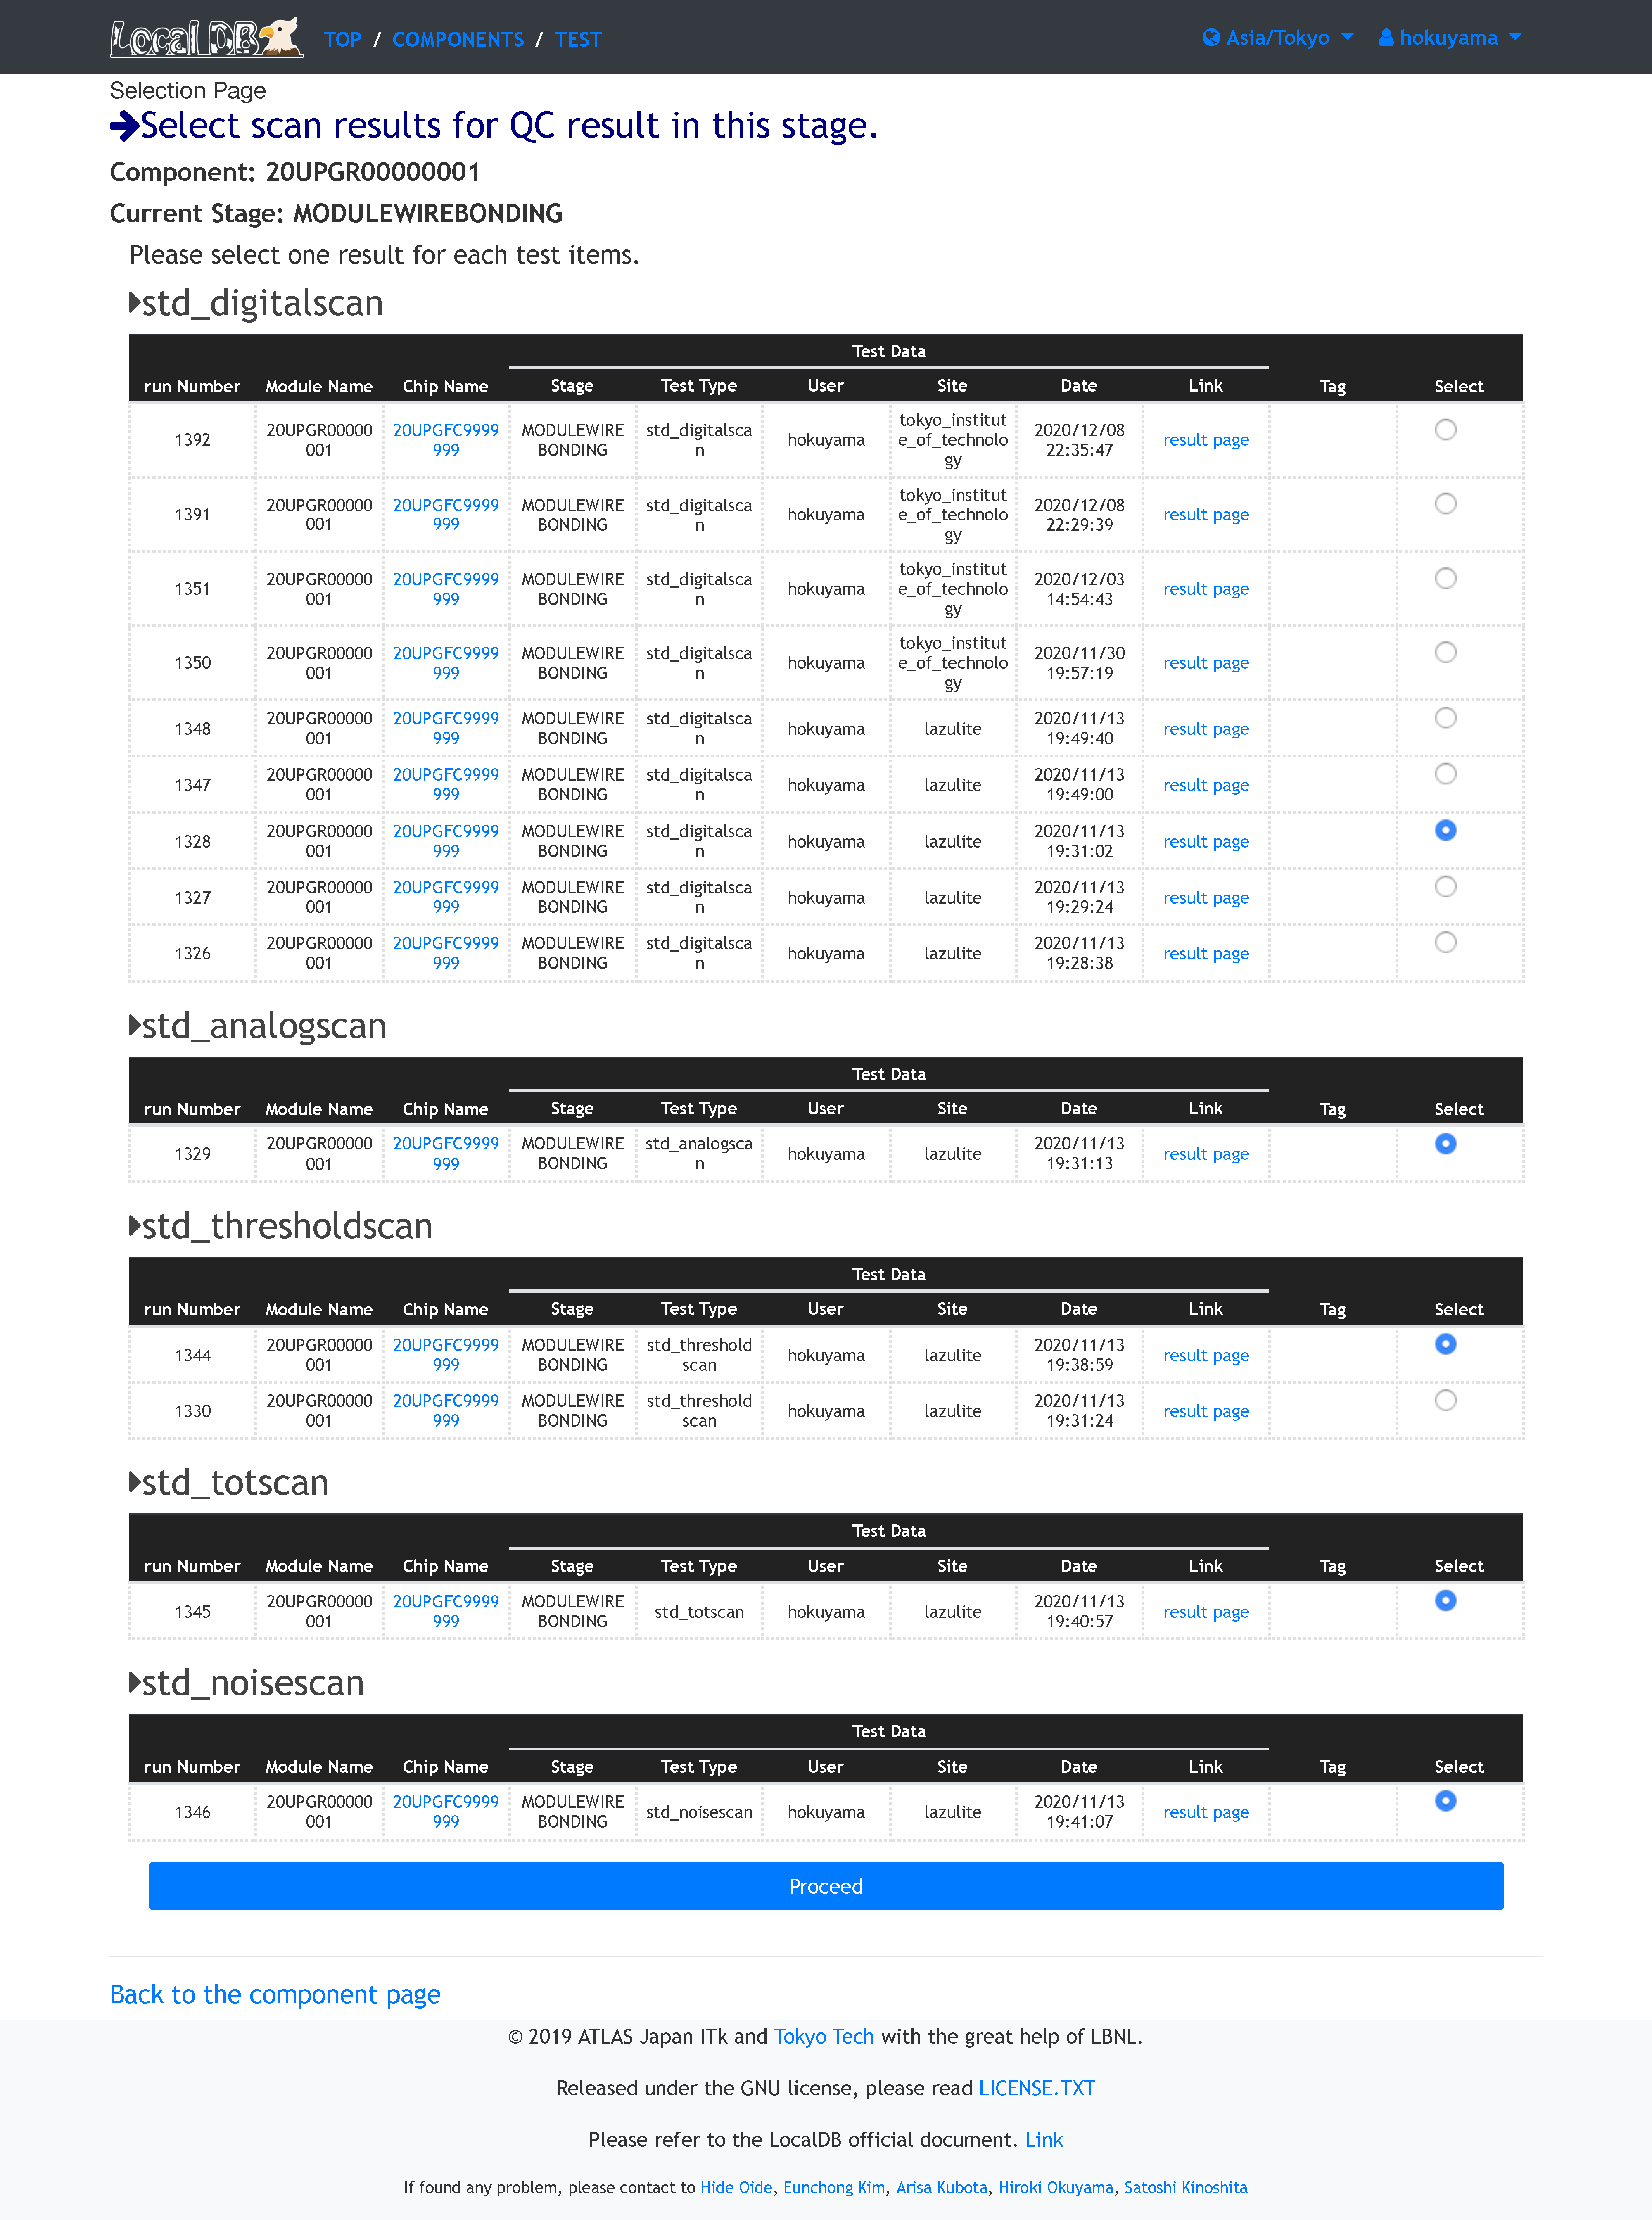
\includegraphics[width=9cm]{demo_select_scans}
  \caption[試験結果の選択]{試験結果の選択}
  \label{demo_select_scans}
  \end{center}
\end{figure}

このデモンストレーションにおける不良評価基準は3章に述べた表\ref{pixel_analysis_criteria}の中から、現時点でシステムに実装している以下の項目を抜粋した。
\begin{enumerate}
  \item Digital Dead 
  \item Digital Bad 
  \item Analog Dead 
  \item Analog Bad 
  \item Tuning Failed
  \item Tuning Bad for Threshold
  \item Tuning Bad for ToT
  \item High ENC
  \item Noisy
\end{enumerate}

解析結果を図\ref{pixel_analysis_result}、それぞれの評価基準における不良ピクセルの分布を図\ref{pixel_analysis_result_dist}に示す。

\begin{figure}[bpt]\centering
\includegraphics[width=12cm]{./data/analysis_result/Bad_Pixels.png}
\caption[ピクセル解析結果]{ピクセル解析結果}
\label{pixel_analysis_result}
\end{figure}

\begin{figure}[bpt]\centering
  \begin{minipage}{0.45\hsize}
    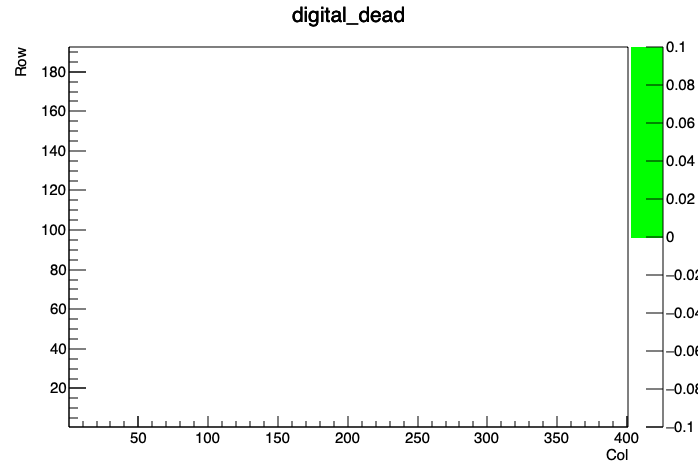
\includegraphics[width=6.5cm]{./data/analysis_result/digital_dead.png}
  \end{minipage}
  \begin{minipage}{0.45\hsize}
    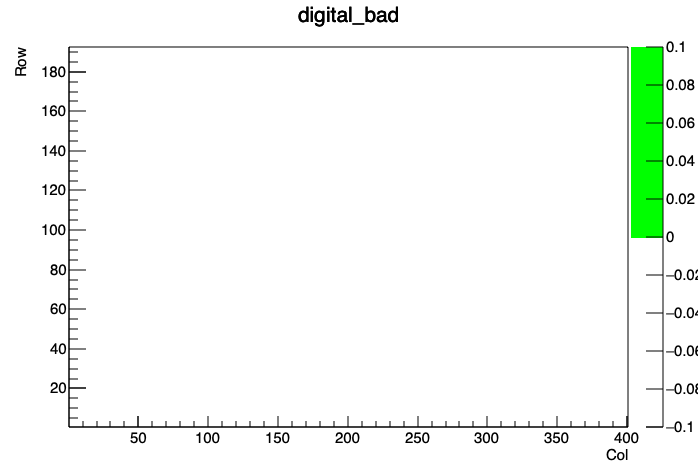
\includegraphics[width=6.5cm]{./data/analysis_result/digital_bad.png}
  \end{minipage}
  \begin{minipage}{0.45\hsize}
    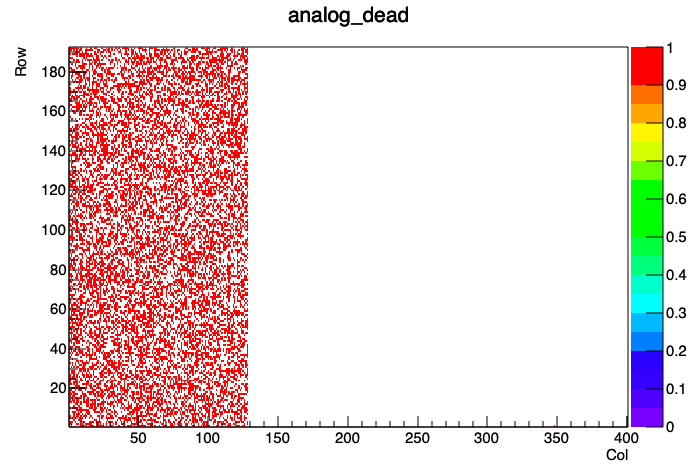
\includegraphics[width=6.5cm]{./data/analysis_result/analog_dead.png}
  \end{minipage}
  \begin{minipage}{0.45\hsize}
    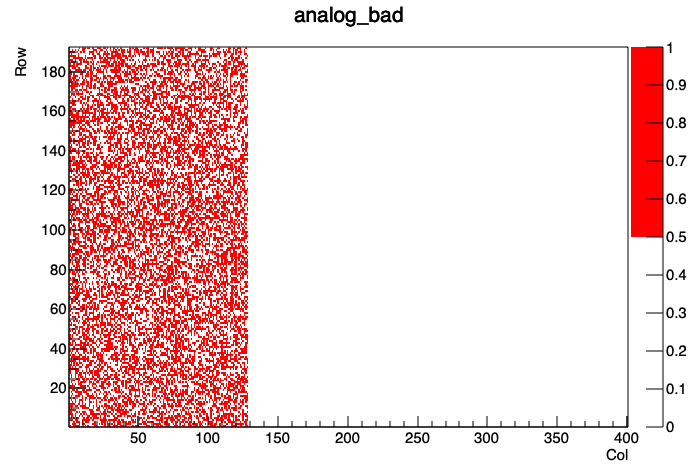
\includegraphics[width=6.5cm]{./data/analysis_result/analog_bad.png}
  \end{minipage}
  \begin{minipage}{0.45\hsize}
    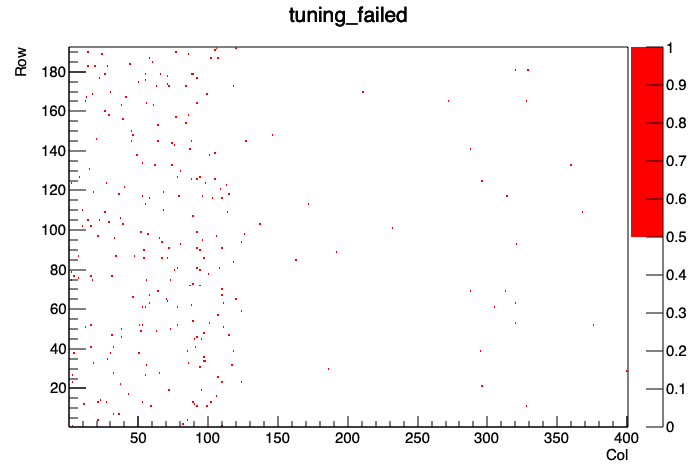
\includegraphics[width=6.5cm]{./data/analysis_result/tuning_failed.png}
  \end{minipage}
  \begin{minipage}{0.45\hsize}
    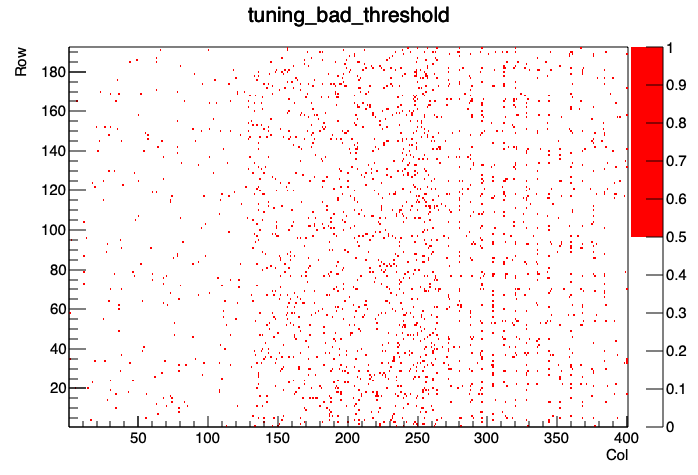
\includegraphics[width=6.5cm]{./data/analysis_result/tuning_bad_threshold.png}
  \end{minipage}
  \begin{minipage}{0.45\hsize}
    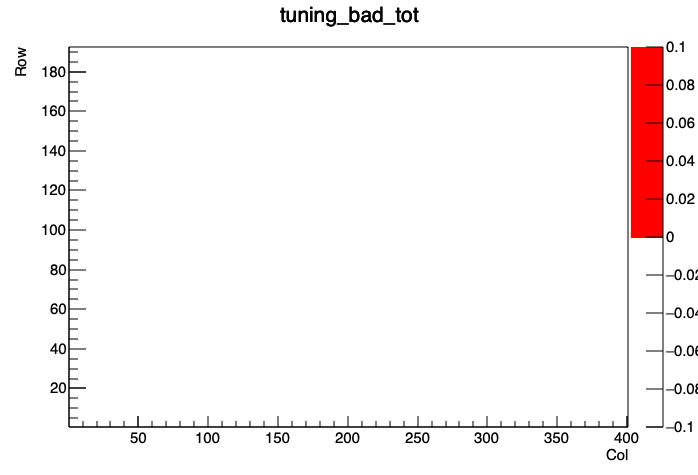
\includegraphics[width=6.5cm]{./data/analysis_result/tuning_bad_tot.png}
  \end{minipage}
  \begin{minipage}{0.45\hsize}
    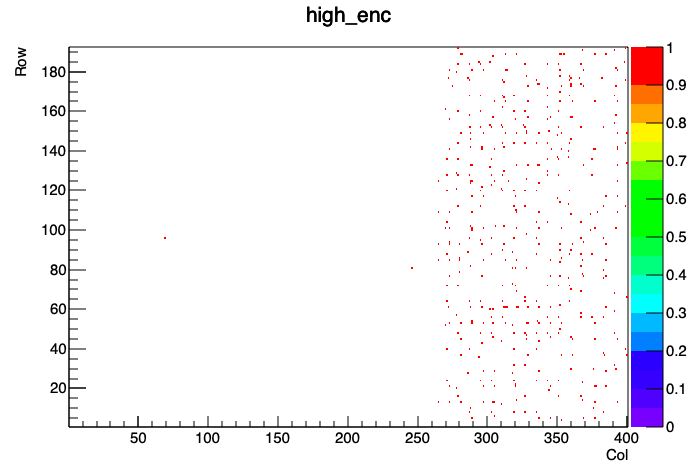
\includegraphics[width=6.5cm]{./data/analysis_result/high_enc.png}
  \end{minipage}
  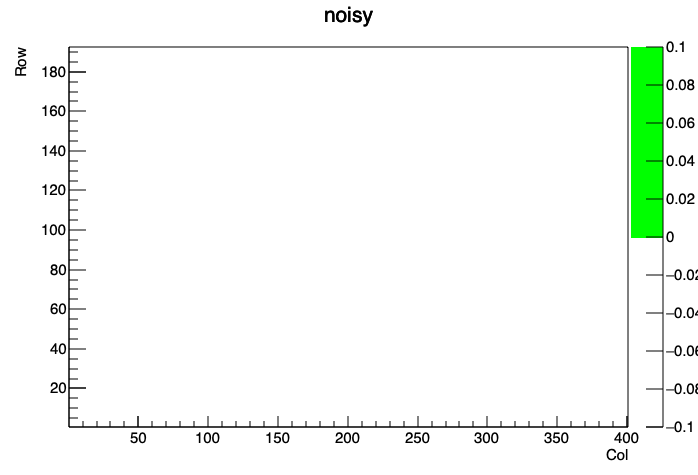
\includegraphics[width=6.5cm]{./data/analysis_result/noisy.png}

\caption[不良ピクセル分布]{不良ピクセル分布}
\label{pixel_analysis_result_figure_dist}
\end{figure}

%%%%%%%%%%%%%%%%%%%%%%%%%%%%%%%%%%%%%%%%%%%%%%%%%
%%%%%%%%%%%%%%%%%%%%%%%%%%%%%%%%%%%%%%%%%%%%%%%%%
\clearpage
\subsubsection{試験結果アップロード}
読み出し試験の結果を解析結果と合わせて中央データベースにアップロードし、情報が正しくアップロードされていることを確認した。
図\ref{demo_upload_to_pd}に中央データベースのウェブページを示す。結果ファイルや解析結果が正しくアップロードされていることが分かる。

\begin{figure}[bpt]\centering
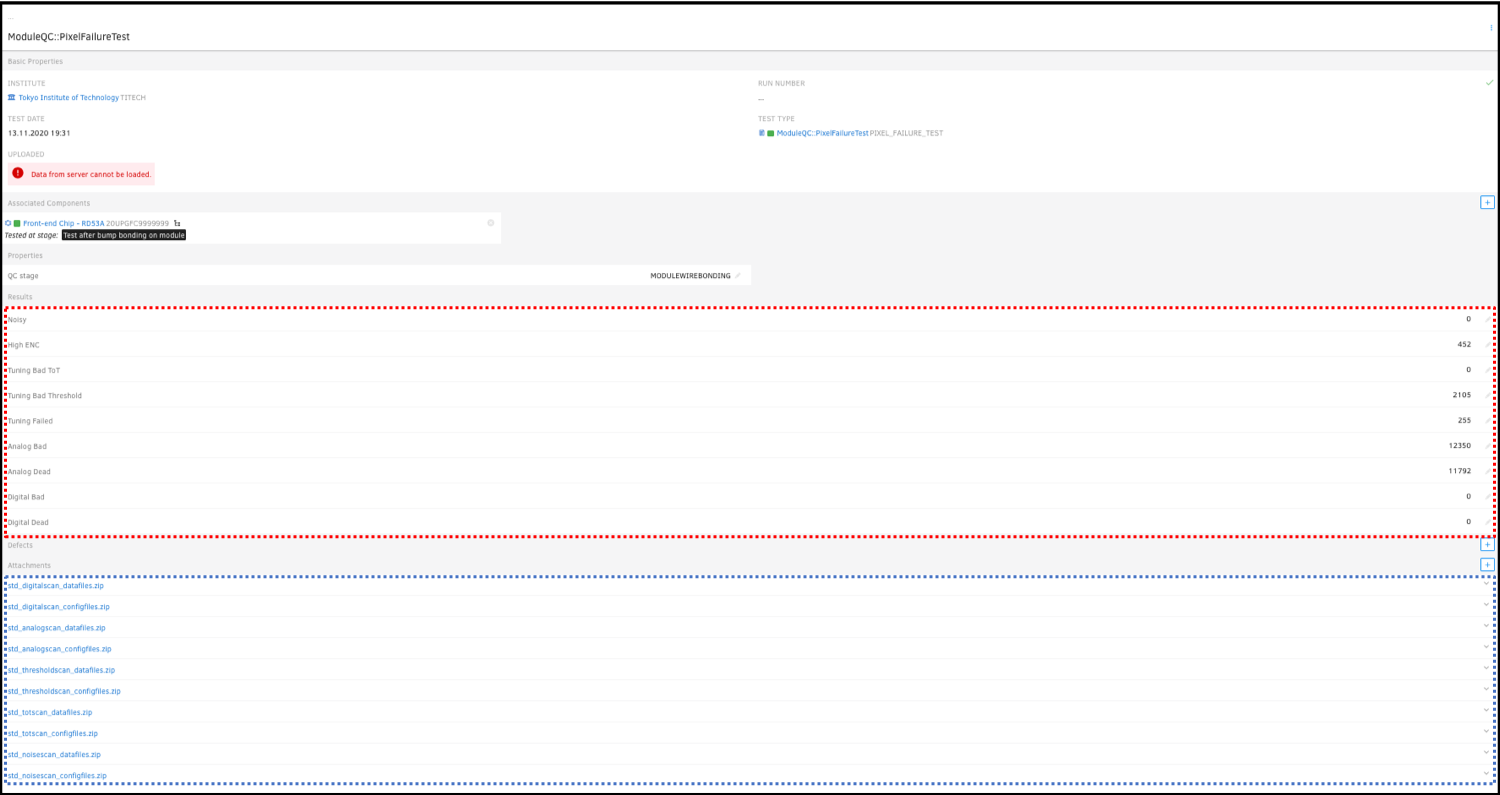
\includegraphics[width=15cm]{demo_upload_to_pd}
\caption[ピクセル解析結果]{ピクセル解析結果}
\label{demo_upload_to_pd}
\end{figure}


